\PassOptionsToPackage{table}{xcolor}
\documentclass[aspectratio=169,11pt,t]{beamer}
\usepackage[russian]{academicbeamer}
\setshorttitle{BelOAI~\textbar~Лекция 4}

\usetikzlibrary{arrows.meta,positioning,decorations.pathreplacing}
\usepackage{pgfplots}
\pgfplotsset{compat=1.18,
  gd end/.style={only marks,mark=*,mark size=1.3pt,mark options={fill=acOrange,draw=acOrange}},
  gd end hidden/.style={only marks,mark=*,mark size=1.3pt,mark options={fill=white,draw=acOrange}}}
\graphicspath{{assets/}}

% Deck-local styling, same as lecture 1.
\definecolor{acOrange}{RGB}{225,115,45}
\colorlet{acAccent}{acMid}
\colorlet{acInk}{acDark}
\colorlet{acCard}{white}
\colorlet{acText}{black!85}
\tikzset{
  chart axis/.style={draw=acGray!70, line width=0.6pt},
  chart label/.style={font=\scriptsize, text=acGray, inner sep=2pt},
  chart curve/.style={draw=acMid, line width=1.2pt, line cap=round},
  level line/.style={draw=acMid!55, line width=0.6pt},
  gd path/.style={draw=acOrange, line width=1pt, line join=round},
  gd point/.style={circle, fill=acOrange, inner sep=0pt, minimum size=3.6pt},
  flow box/.style={rectangle, rounded corners=2pt, minimum height=0.85cm, inner xsep=6pt,
    text=white, font=\small\bfseries, align=center},
  flow arrow/.style={-{Stealth[length=2.2mm]}, line width=1.1pt, color=acGray}
}

% Zebra tables in the theme palette: \zebra{first-shaded-row} before a tabular.
\newcommand{\zebra}[1]{\rowcolors{#1}{acLight}{white}\renewcommand{\arraystretch}{1.45}\setlength{\tabcolsep}{7pt}\normalsize}

% Numbered rows: \begin{numrows} 1 & text\\ ... \end{numrows}
\newenvironment{numrows}{\zebra{1}\begin{tabular}{>{\bfseries\large\color{acMid}}c >{\raggedright\arraybackslash}p{\dimexpr\linewidth-1.7cm\relax}}}{\end{tabular}}

% Ragged-right text: no stretched word spacing or ugly hyphenation in narrow blocks.
\usepackage{ragged2e}
\addtobeamertemplate{block begin}{}{\advance\rightskip 0pt plus 4em\relax}
\setbeamerfont{block title}{size=\normalsize,series=\bfseries}
\setbeamerfont{block body}{size=\normalsize}
\hyphenpenalty=10000
\exhyphenpenalty=10000

\title{Как учится модель}
\subtitle{Данные, проверка качества, производные и градиентный спуск}
\author{Алексей Чернуха}
\date{24 октября 2026}

\begin{document}

\begin{frame}[plain]
  \vspace{1.1cm}
  \hspace{0.02\paperwidth}\begin{minipage}{0.9\paperwidth}
  {\color{acRule}\hrule height 0.9pt}\vspace{0.8em}
  {\usebeamerfont{title}\usebeamercolor[fg]{title}\inserttitle\par}
  \vspace{0.7em}
  {\large\color{acMid}\insertsubtitle\par}
  \vspace{0.8em}{\color{acRule}\hrule height 0.9pt}
  \vspace{1.4em}
  {\small\color{acGray}\insertauthor\par}
  \vspace{0.9em}
  {\small\color{acGray}\insertdate}
  \end{minipage}
\end{frame}

\section{Повторение}

\begin{frame}[c]{Что было на прошлой неделе}
  \begin{columns}[T]
    \begin{column}{0.47\textwidth}
      \centering
      \begin{tikzpicture}[x=0.75cm,y=0.55cm]
        \draw[chart axis] (-0.3,0) -- (6.3,0) node[chart label,anchor=west] {$w$};
        \draw[chart axis] (0,-0.3) -- (0,5.2) node[chart label,anchor=south] {MSE};
        \draw[chart curve,domain=0.2:5.8,samples=60] plot (\x,{0.5*(\x-3)^2+0.6});
        % tangent at w=1: slope -2
        \draw[acOrange,line width=0.9pt,dashed] (0.2,4.2) -- (2.2,0.2);
        \fill[acOrange] (1,2.6) circle (2.4pt);
        \node[chart label,anchor=west] at (1.1,2.75) {$w_k$};
        \draw[-{Stealth[length=2mm]},acOrange,line width=1.1pt] (1,-0.7) -- (2.4,-0.7);
        \node[chart label,anchor=north,text=acOrange] at (1.7,-0.75) {шаг $-\eta\,L'(w_k)$};
        \draw[acOrange!60,dashed] (1,2.6) -- (1,-0.7);
        \fill[acDark] (3,0.6) circle (2pt);
        \node[chart label,anchor=north] at (3.3,0.45) {минимум};
      \end{tikzpicture}
    \end{column}
    \begin{column}{0.49\textwidth}
      \begin{block}{Линейная регрессия}
        \small
        Модель $\hat y = w x + b$, ошибка
        $\mathrm{MSE}=\frac1n\sum (\hat y_i-y_i)^2$.
      \end{block}
      \begin{block}{Градиентный спуск в 1D}
        \small
        \centerline{$w_{k+1} = w_k - \eta\,L'(w_k)$}
        \smallskip
        Производная показывает наклон. Идём в сторону убывания, шаг $\eta$ выбираем сами:
        маленький --- медленно, большой --- разлетаемся.
      \end{block}
    \end{column}
  \end{columns}

  \medskip
  \lead{Сегодня:} откуда берутся данные, как честно проверить модель и как считать градиент,
  когда параметров много.
\end{frame}

\section{Откуда берутся датасеты}

\begin{frame}[c]{Откуда берутся данные}
  \begin{columns}[T]
    \begin{column}{0.23\textwidth}
      \begin{block}{Готовые}
        \small
        Kaggle, Hugging Face, UCI. Быстро, но задачу за вас уже кто-то сформулировал.
      \end{block}
    \end{column}
    \begin{column}{0.23\textwidth}
      \begin{block}{Собранные}
        \small
        Логи сервиса, парсинг сайтов, датчики, фото на телефон.
      \end{block}
    \end{column}
    \begin{column}{0.23\textwidth}
      \begin{block}{Размеченные}
        \small
        Объекты есть, ответов нет. Ответы ставят люди: эксперты или краудсорсинг.
      \end{block}
    \end{column}
    \begin{column}{0.23\textwidth}
      \begin{block}{Синтетические}
        \small
        Сгенерированы по формуле или другой моделью.
      \end{block}
    \end{column}
  \end{columns}

  \medskip
  \lead{Чаще всего самое долгое в ML-проекте --- не обучение, а сбор и чистка данных.}
\end{frame}

\begin{frame}[c]{MNIST: рукописные цифры}
  \begin{columns}[T]
    \begin{column}{0.50\textwidth}
      \centering
      % Handwritten digits 8x8 from the UCI Optical Recognition of Handwritten Digits
% dataset (copy shipped with scikit-learn, digits.csv.gz). Two samples per digit.
\begin{tikzpicture}[x=0.075cm,y=0.075cm]
  \fill[acLight] (0.0,0.0) rectangle ++(8,-8);
  \fill[acDark!31!acLight] (2.0,0.0) rectangle ++(1,-1);
  \fill[acDark!81!acLight] (3.0,0.0) rectangle ++(1,-1);
  \fill[acDark!56!acLight] (4.0,0.0) rectangle ++(1,-1);
  \fill[acDark!6!acLight] (5.0,0.0) rectangle ++(1,-1);
  \fill[acDark!81!acLight] (2.0,-1.0) rectangle ++(1,-1);
  \fill[acDark!93!acLight] (3.0,-1.0) rectangle ++(1,-1);
  \fill[acDark!62!acLight] (4.0,-1.0) rectangle ++(1,-1);
  \fill[acDark!93!acLight] (5.0,-1.0) rectangle ++(1,-1);
  \fill[acDark!31!acLight] (6.0,-1.0) rectangle ++(1,-1);
  \fill[acDark!18!acLight] (1.0,-2.0) rectangle ++(1,-1);
  \fill[acDark!93!acLight] (2.0,-2.0) rectangle ++(1,-1);
  \fill[acDark!12!acLight] (3.0,-2.0) rectangle ++(1,-1);
  \fill[acDark!68!acLight] (5.0,-2.0) rectangle ++(1,-1);
  \fill[acDark!50!acLight] (6.0,-2.0) rectangle ++(1,-1);
  \fill[acDark!25!acLight] (1.0,-3.0) rectangle ++(1,-1);
  \fill[acDark!75!acLight] (2.0,-3.0) rectangle ++(1,-1);
  \fill[acDark!50!acLight] (5.0,-3.0) rectangle ++(1,-1);
  \fill[acDark!50!acLight] (6.0,-3.0) rectangle ++(1,-1);
  \fill[acDark!31!acLight] (1.0,-4.0) rectangle ++(1,-1);
  \fill[acDark!50!acLight] (2.0,-4.0) rectangle ++(1,-1);
  \fill[acDark!56!acLight] (5.0,-4.0) rectangle ++(1,-1);
  \fill[acDark!50!acLight] (6.0,-4.0) rectangle ++(1,-1);
  \fill[acDark!25!acLight] (1.0,-5.0) rectangle ++(1,-1);
  \fill[acDark!68!acLight] (2.0,-5.0) rectangle ++(1,-1);
  \fill[acDark!6!acLight] (4.0,-5.0) rectangle ++(1,-1);
  \fill[acDark!75!acLight] (5.0,-5.0) rectangle ++(1,-1);
  \fill[acDark!43!acLight] (6.0,-5.0) rectangle ++(1,-1);
  \fill[acDark!12!acLight] (1.0,-6.0) rectangle ++(1,-1);
  \fill[acDark!87!acLight] (2.0,-6.0) rectangle ++(1,-1);
  \fill[acDark!31!acLight] (3.0,-6.0) rectangle ++(1,-1);
  \fill[acDark!62!acLight] (4.0,-6.0) rectangle ++(1,-1);
  \fill[acDark!75!acLight] (5.0,-6.0) rectangle ++(1,-1);
  \fill[acDark!37!acLight] (2.0,-7.0) rectangle ++(1,-1);
  \fill[acDark!81!acLight] (3.0,-7.0) rectangle ++(1,-1);
  \fill[acDark!62!acLight] (4.0,-7.0) rectangle ++(1,-1);
  \fill[acLight] (9.5,0.0) rectangle ++(8,-8);
  \fill[acDark!75!acLight] (12.5,0.0) rectangle ++(1,-1);
  \fill[acDark!81!acLight] (13.5,0.0) rectangle ++(1,-1);
  \fill[acDark!31!acLight] (14.5,0.0) rectangle ++(1,-1);
  \fill[acDark!68!acLight] (12.5,-1.0) rectangle ++(1,-1);
  \fill[acDark!100!acLight] (13.5,-1.0) rectangle ++(1,-1);
  \fill[acDark!56!acLight] (14.5,-1.0) rectangle ++(1,-1);
  \fill[acDark!18!acLight] (11.5,-2.0) rectangle ++(1,-1);
  \fill[acDark!93!acLight] (12.5,-2.0) rectangle ++(1,-1);
  \fill[acDark!100!acLight] (13.5,-2.0) rectangle ++(1,-1);
  \fill[acDark!37!acLight] (14.5,-2.0) rectangle ++(1,-1);
  \fill[acDark!43!acLight] (10.5,-3.0) rectangle ++(1,-1);
  \fill[acDark!93!acLight] (11.5,-3.0) rectangle ++(1,-1);
  \fill[acDark!100!acLight] (12.5,-3.0) rectangle ++(1,-1);
  \fill[acDark!100!acLight] (13.5,-3.0) rectangle ++(1,-1);
  \fill[acDark!12!acLight] (14.5,-3.0) rectangle ++(1,-1);
  \fill[acDark!6!acLight] (11.5,-4.0) rectangle ++(1,-1);
  \fill[acDark!100!acLight] (12.5,-4.0) rectangle ++(1,-1);
  \fill[acDark!100!acLight] (13.5,-4.0) rectangle ++(1,-1);
  \fill[acDark!18!acLight] (14.5,-4.0) rectangle ++(1,-1);
  \fill[acDark!6!acLight] (11.5,-5.0) rectangle ++(1,-1);
  \fill[acDark!100!acLight] (12.5,-5.0) rectangle ++(1,-1);
  \fill[acDark!100!acLight] (13.5,-5.0) rectangle ++(1,-1);
  \fill[acDark!37!acLight] (14.5,-5.0) rectangle ++(1,-1);
  \fill[acDark!6!acLight] (11.5,-6.0) rectangle ++(1,-1);
  \fill[acDark!100!acLight] (12.5,-6.0) rectangle ++(1,-1);
  \fill[acDark!100!acLight] (13.5,-6.0) rectangle ++(1,-1);
  \fill[acDark!37!acLight] (14.5,-6.0) rectangle ++(1,-1);
  \fill[acDark!68!acLight] (12.5,-7.0) rectangle ++(1,-1);
  \fill[acDark!100!acLight] (13.5,-7.0) rectangle ++(1,-1);
  \fill[acDark!62!acLight] (14.5,-7.0) rectangle ++(1,-1);
  \fill[acLight] (19.0,0.0) rectangle ++(8,-8);
  \fill[acDark!25!acLight] (22.0,0.0) rectangle ++(1,-1);
  \fill[acDark!93!acLight] (23.0,0.0) rectangle ++(1,-1);
  \fill[acDark!75!acLight] (24.0,0.0) rectangle ++(1,-1);
  \fill[acDark!18!acLight] (21.0,-1.0) rectangle ++(1,-1);
  \fill[acDark!100!acLight] (22.0,-1.0) rectangle ++(1,-1);
  \fill[acDark!93!acLight] (23.0,-1.0) rectangle ++(1,-1);
  \fill[acDark!87!acLight] (24.0,-1.0) rectangle ++(1,-1);
  \fill[acDark!50!acLight] (21.0,-2.0) rectangle ++(1,-1);
  \fill[acDark!81!acLight] (22.0,-2.0) rectangle ++(1,-1);
  \fill[acDark!50!acLight] (23.0,-2.0) rectangle ++(1,-1);
  \fill[acDark!100!acLight] (24.0,-2.0) rectangle ++(1,-1);
  \fill[acDark!6!acLight] (21.0,-3.0) rectangle ++(1,-1);
  \fill[acDark!37!acLight] (22.0,-3.0) rectangle ++(1,-1);
  \fill[acDark!93!acLight] (23.0,-3.0) rectangle ++(1,-1);
  \fill[acDark!68!acLight] (24.0,-3.0) rectangle ++(1,-1);
  \fill[acDark!6!acLight] (20.0,-4.0) rectangle ++(1,-1);
  \fill[acDark!50!acLight] (21.0,-4.0) rectangle ++(1,-1);
  \fill[acDark!81!acLight] (22.0,-4.0) rectangle ++(1,-1);
  \fill[acDark!93!acLight] (23.0,-4.0) rectangle ++(1,-1);
  \fill[acDark!6!acLight] (24.0,-4.0) rectangle ++(1,-1);
  \fill[acDark!56!acLight] (20.0,-5.0) rectangle ++(1,-1);
  \fill[acDark!100!acLight] (21.0,-5.0) rectangle ++(1,-1);
  \fill[acDark!100!acLight] (22.0,-5.0) rectangle ++(1,-1);
  \fill[acDark!31!acLight] (23.0,-5.0) rectangle ++(1,-1);
  \fill[acDark!18!acLight] (20.0,-6.0) rectangle ++(1,-1);
  \fill[acDark!81!acLight] (21.0,-6.0) rectangle ++(1,-1);
  \fill[acDark!100!acLight] (22.0,-6.0) rectangle ++(1,-1);
  \fill[acDark!100!acLight] (23.0,-6.0) rectangle ++(1,-1);
  \fill[acDark!68!acLight] (24.0,-6.0) rectangle ++(1,-1);
  \fill[acDark!31!acLight] (25.0,-6.0) rectangle ++(1,-1);
  \fill[acDark!18!acLight] (22.0,-7.0) rectangle ++(1,-1);
  \fill[acDark!68!acLight] (23.0,-7.0) rectangle ++(1,-1);
  \fill[acDark!100!acLight] (24.0,-7.0) rectangle ++(1,-1);
  \fill[acDark!56!acLight] (25.0,-7.0) rectangle ++(1,-1);
  \fill[acLight] (28.5,0.0) rectangle ++(8,-8);
  \fill[acDark!43!acLight] (30.5,0.0) rectangle ++(1,-1);
  \fill[acDark!93!acLight] (31.5,0.0) rectangle ++(1,-1);
  \fill[acDark!81!acLight] (32.5,0.0) rectangle ++(1,-1);
  \fill[acDark!6!acLight] (33.5,0.0) rectangle ++(1,-1);
  \fill[acDark!50!acLight] (29.5,-1.0) rectangle ++(1,-1);
  \fill[acDark!81!acLight] (30.5,-1.0) rectangle ++(1,-1);
  \fill[acDark!37!acLight] (31.5,-1.0) rectangle ++(1,-1);
  \fill[acDark!93!acLight] (32.5,-1.0) rectangle ++(1,-1);
  \fill[acDark!25!acLight] (33.5,-1.0) rectangle ++(1,-1);
  \fill[acDark!12!acLight] (29.5,-2.0) rectangle ++(1,-1);
  \fill[acDark!6!acLight] (30.5,-2.0) rectangle ++(1,-1);
  \fill[acDark!81!acLight] (31.5,-2.0) rectangle ++(1,-1);
  \fill[acDark!81!acLight] (32.5,-2.0) rectangle ++(1,-1);
  \fill[acDark!12!acLight] (30.5,-3.0) rectangle ++(1,-1);
  \fill[acDark!93!acLight] (31.5,-3.0) rectangle ++(1,-1);
  \fill[acDark!68!acLight] (32.5,-3.0) rectangle ++(1,-1);
  \fill[acDark!6!acLight] (33.5,-3.0) rectangle ++(1,-1);
  \fill[acDark!6!acLight] (31.5,-4.0) rectangle ++(1,-1);
  \fill[acDark!75!acLight] (32.5,-4.0) rectangle ++(1,-1);
  \fill[acDark!75!acLight] (33.5,-4.0) rectangle ++(1,-1);
  \fill[acDark!6!acLight] (34.5,-4.0) rectangle ++(1,-1);
  \fill[acDark!6!acLight] (32.5,-5.0) rectangle ++(1,-1);
  \fill[acDark!62!acLight] (33.5,-5.0) rectangle ++(1,-1);
  \fill[acDark!50!acLight] (34.5,-5.0) rectangle ++(1,-1);
  \fill[acDark!50!acLight] (30.5,-6.0) rectangle ++(1,-1);
  \fill[acDark!25!acLight] (31.5,-6.0) rectangle ++(1,-1);
  \fill[acDark!31!acLight] (32.5,-6.0) rectangle ++(1,-1);
  \fill[acDark!87!acLight] (33.5,-6.0) rectangle ++(1,-1);
  \fill[acDark!56!acLight] (34.5,-6.0) rectangle ++(1,-1);
  \fill[acDark!43!acLight] (30.5,-7.0) rectangle ++(1,-1);
  \fill[acDark!81!acLight] (31.5,-7.0) rectangle ++(1,-1);
  \fill[acDark!81!acLight] (32.5,-7.0) rectangle ++(1,-1);
  \fill[acDark!56!acLight] (33.5,-7.0) rectangle ++(1,-1);
  \fill[acLight] (38.0,0.0) rectangle ++(8,-8);
  \fill[acDark!6!acLight] (41.0,0.0) rectangle ++(1,-1);
  \fill[acDark!68!acLight] (42.0,0.0) rectangle ++(1,-1);
  \fill[acDark!43!acLight] (41.0,-1.0) rectangle ++(1,-1);
  \fill[acDark!50!acLight] (42.0,-1.0) rectangle ++(1,-1);
  \fill[acDark!6!acLight] (40.0,-2.0) rectangle ++(1,-1);
  \fill[acDark!81!acLight] (41.0,-2.0) rectangle ++(1,-1);
  \fill[acDark!37!acLight] (42.0,-2.0) rectangle ++(1,-1);
  \fill[acDark!12!acLight] (43.0,-2.0) rectangle ++(1,-1);
  \fill[acDark!12!acLight] (44.0,-2.0) rectangle ++(1,-1);
  \fill[acDark!43!acLight] (40.0,-3.0) rectangle ++(1,-1);
  \fill[acDark!93!acLight] (41.0,-3.0) rectangle ++(1,-1);
  \fill[acDark!56!acLight] (43.0,-3.0) rectangle ++(1,-1);
  \fill[acDark!50!acLight] (44.0,-3.0) rectangle ++(1,-1);
  \fill[acDark!31!acLight] (39.0,-4.0) rectangle ++(1,-1);
  \fill[acDark!100!acLight] (40.0,-4.0) rectangle ++(1,-1);
  \fill[acDark!62!acLight] (41.0,-4.0) rectangle ++(1,-1);
  \fill[acDark!100!acLight] (43.0,-4.0) rectangle ++(1,-1);
  \fill[acDark!37!acLight] (44.0,-4.0) rectangle ++(1,-1);
  \fill[acDark!25!acLight] (39.0,-5.0) rectangle ++(1,-1);
  \fill[acDark!93!acLight] (40.0,-5.0) rectangle ++(1,-1);
  \fill[acDark!100!acLight] (41.0,-5.0) rectangle ++(1,-1);
  \fill[acDark!81!acLight] (42.0,-5.0) rectangle ++(1,-1);
  \fill[acDark!100!acLight] (43.0,-5.0) rectangle ++(1,-1);
  \fill[acDark!6!acLight] (44.0,-5.0) rectangle ++(1,-1);
  \fill[acDark!18!acLight] (41.0,-6.0) rectangle ++(1,-1);
  \fill[acDark!93!acLight] (42.0,-6.0) rectangle ++(1,-1);
  \fill[acDark!62!acLight] (43.0,-6.0) rectangle ++(1,-1);
  \fill[acDark!12!acLight] (41.0,-7.0) rectangle ++(1,-1);
  \fill[acDark!100!acLight] (42.0,-7.0) rectangle ++(1,-1);
  \fill[acDark!25!acLight] (43.0,-7.0) rectangle ++(1,-1);
  \fill[acLight] (47.5,0.0) rectangle ++(8,-8);
  \fill[acDark!75!acLight] (49.5,0.0) rectangle ++(1,-1);
  \fill[acDark!62!acLight] (50.5,0.0) rectangle ++(1,-1);
  \fill[acDark!87!acLight] (49.5,-1.0) rectangle ++(1,-1);
  \fill[acDark!100!acLight] (50.5,-1.0) rectangle ++(1,-1);
  \fill[acDark!100!acLight] (51.5,-1.0) rectangle ++(1,-1);
  \fill[acDark!87!acLight] (52.5,-1.0) rectangle ++(1,-1);
  \fill[acDark!81!acLight] (49.5,-2.0) rectangle ++(1,-1);
  \fill[acDark!100!acLight] (50.5,-2.0) rectangle ++(1,-1);
  \fill[acDark!93!acLight] (51.5,-2.0) rectangle ++(1,-1);
  \fill[acDark!62!acLight] (52.5,-2.0) rectangle ++(1,-1);
  \fill[acDark!6!acLight] (53.5,-2.0) rectangle ++(1,-1);
  \fill[acDark!68!acLight] (49.5,-3.0) rectangle ++(1,-1);
  \fill[acDark!100!acLight] (50.5,-3.0) rectangle ++(1,-1);
  \fill[acDark!100!acLight] (51.5,-3.0) rectangle ++(1,-1);
  \fill[acDark!43!acLight] (52.5,-3.0) rectangle ++(1,-1);
  \fill[acDark!25!acLight] (50.5,-4.0) rectangle ++(1,-1);
  \fill[acDark!43!acLight] (51.5,-4.0) rectangle ++(1,-1);
  \fill[acDark!100!acLight] (52.5,-4.0) rectangle ++(1,-1);
  \fill[acDark!43!acLight] (53.5,-4.0) rectangle ++(1,-1);
  \fill[acDark!25!acLight] (51.5,-5.0) rectangle ++(1,-1);
  \fill[acDark!100!acLight] (52.5,-5.0) rectangle ++(1,-1);
  \fill[acDark!56!acLight] (53.5,-5.0) rectangle ++(1,-1);
  \fill[acDark!31!acLight] (49.5,-6.0) rectangle ++(1,-1);
  \fill[acDark!25!acLight] (50.5,-6.0) rectangle ++(1,-1);
  \fill[acDark!75!acLight] (51.5,-6.0) rectangle ++(1,-1);
  \fill[acDark!100!acLight] (52.5,-6.0) rectangle ++(1,-1);
  \fill[acDark!25!acLight] (53.5,-6.0) rectangle ++(1,-1);
  \fill[acDark!56!acLight] (49.5,-7.0) rectangle ++(1,-1);
  \fill[acDark!100!acLight] (50.5,-7.0) rectangle ++(1,-1);
  \fill[acDark!100!acLight] (51.5,-7.0) rectangle ++(1,-1);
  \fill[acDark!62!acLight] (52.5,-7.0) rectangle ++(1,-1);
  \fill[acLight] (57.0,0.0) rectangle ++(8,-8);
  \fill[acDark!75!acLight] (60.0,0.0) rectangle ++(1,-1);
  \fill[acDark!81!acLight] (61.0,0.0) rectangle ++(1,-1);
  \fill[acDark!31!acLight] (59.0,-1.0) rectangle ++(1,-1);
  \fill[acDark!100!acLight] (60.0,-1.0) rectangle ++(1,-1);
  \fill[acDark!50!acLight] (61.0,-1.0) rectangle ++(1,-1);
  \fill[acDark!81!acLight] (59.0,-2.0) rectangle ++(1,-1);
  \fill[acDark!100!acLight] (60.0,-2.0) rectangle ++(1,-1);
  \fill[acDark!18!acLight] (61.0,-2.0) rectangle ++(1,-1);
  \fill[acDark!87!acLight] (59.0,-3.0) rectangle ++(1,-1);
  \fill[acDark!81!acLight] (60.0,-3.0) rectangle ++(1,-1);
  \fill[acDark!93!acLight] (59.0,-4.0) rectangle ++(1,-1);
  \fill[acDark!75!acLight] (60.0,-4.0) rectangle ++(1,-1);
  \fill[acDark!43!acLight] (61.0,-4.0) rectangle ++(1,-1);
  \fill[acDark!12!acLight] (62.0,-4.0) rectangle ++(1,-1);
  \fill[acDark!81!acLight] (59.0,-5.0) rectangle ++(1,-1);
  \fill[acDark!100!acLight] (60.0,-5.0) rectangle ++(1,-1);
  \fill[acDark!81!acLight] (61.0,-5.0) rectangle ++(1,-1);
  \fill[acDark!100!acLight] (62.0,-5.0) rectangle ++(1,-1);
  \fill[acDark!18!acLight] (63.0,-5.0) rectangle ++(1,-1);
  \fill[acDark!43!acLight] (59.0,-6.0) rectangle ++(1,-1);
  \fill[acDark!100!acLight] (60.0,-6.0) rectangle ++(1,-1);
  \fill[acDark!68!acLight] (61.0,-6.0) rectangle ++(1,-1);
  \fill[acDark!93!acLight] (62.0,-6.0) rectangle ++(1,-1);
  \fill[acDark!50!acLight] (63.0,-6.0) rectangle ++(1,-1);
  \fill[acDark!6!acLight] (59.0,-7.0) rectangle ++(1,-1);
  \fill[acDark!56!acLight] (60.0,-7.0) rectangle ++(1,-1);
  \fill[acDark!93!acLight] (61.0,-7.0) rectangle ++(1,-1);
  \fill[acDark!68!acLight] (62.0,-7.0) rectangle ++(1,-1);
  \fill[acDark!18!acLight] (63.0,-7.0) rectangle ++(1,-1);
  \fill[acLight] (66.5,0.0) rectangle ++(8,-8);
  \fill[acDark!43!acLight] (68.5,0.0) rectangle ++(1,-1);
  \fill[acDark!50!acLight] (69.5,0.0) rectangle ++(1,-1);
  \fill[acDark!81!acLight] (70.5,0.0) rectangle ++(1,-1);
  \fill[acDark!100!acLight] (71.5,0.0) rectangle ++(1,-1);
  \fill[acDark!93!acLight] (72.5,0.0) rectangle ++(1,-1);
  \fill[acDark!6!acLight] (73.5,0.0) rectangle ++(1,-1);
  \fill[acDark!43!acLight] (68.5,-1.0) rectangle ++(1,-1);
  \fill[acDark!43!acLight] (69.5,-1.0) rectangle ++(1,-1);
  \fill[acDark!25!acLight] (70.5,-1.0) rectangle ++(1,-1);
  \fill[acDark!68!acLight] (71.5,-1.0) rectangle ++(1,-1);
  \fill[acDark!75!acLight] (72.5,-1.0) rectangle ++(1,-1);
  \fill[acDark!50!acLight] (70.5,-2.0) rectangle ++(1,-1);
  \fill[acDark!81!acLight] (71.5,-2.0) rectangle ++(1,-1);
  \fill[acDark!6!acLight] (72.5,-2.0) rectangle ++(1,-1);
  \fill[acDark!25!acLight] (67.5,-3.0) rectangle ++(1,-1);
  \fill[acDark!50!acLight] (68.5,-3.0) rectangle ++(1,-1);
  \fill[acDark!50!acLight] (69.5,-3.0) rectangle ++(1,-1);
  \fill[acDark!93!acLight] (70.5,-3.0) rectangle ++(1,-1);
  \fill[acDark!93!acLight] (71.5,-3.0) rectangle ++(1,-1);
  \fill[acDark!37!acLight] (72.5,-3.0) rectangle ++(1,-1);
  \fill[acDark!12!acLight] (67.5,-4.0) rectangle ++(1,-1);
  \fill[acDark!68!acLight] (68.5,-4.0) rectangle ++(1,-1);
  \fill[acDark!93!acLight] (69.5,-4.0) rectangle ++(1,-1);
  \fill[acDark!93!acLight] (70.5,-4.0) rectangle ++(1,-1);
  \fill[acDark!25!acLight] (71.5,-4.0) rectangle ++(1,-1);
  \fill[acDark!100!acLight] (69.5,-5.0) rectangle ++(1,-1);
  \fill[acDark!31!acLight] (70.5,-5.0) rectangle ++(1,-1);
  \fill[acDark!56!acLight] (68.5,-6.0) rectangle ++(1,-1);
  \fill[acDark!93!acLight] (69.5,-6.0) rectangle ++(1,-1);
  \fill[acDark!6!acLight] (70.5,-6.0) rectangle ++(1,-1);
  \fill[acDark!81!acLight] (68.5,-7.0) rectangle ++(1,-1);
  \fill[acDark!31!acLight] (69.5,-7.0) rectangle ++(1,-1);
  \fill[acLight] (76.0,0.0) rectangle ++(8,-8);
  \fill[acDark!56!acLight] (78.0,0.0) rectangle ++(1,-1);
  \fill[acDark!87!acLight] (79.0,0.0) rectangle ++(1,-1);
  \fill[acDark!50!acLight] (80.0,0.0) rectangle ++(1,-1);
  \fill[acDark!6!acLight] (81.0,0.0) rectangle ++(1,-1);
  \fill[acDark!75!acLight] (78.0,-1.0) rectangle ++(1,-1);
  \fill[acDark!87!acLight] (79.0,-1.0) rectangle ++(1,-1);
  \fill[acDark!87!acLight] (80.0,-1.0) rectangle ++(1,-1);
  \fill[acDark!75!acLight] (81.0,-1.0) rectangle ++(1,-1);
  \fill[acDark!56!acLight] (78.0,-2.0) rectangle ++(1,-1);
  \fill[acDark!62!acLight] (79.0,-2.0) rectangle ++(1,-1);
  \fill[acDark!93!acLight] (81.0,-2.0) rectangle ++(1,-1);
  \fill[acDark!25!acLight] (82.0,-2.0) rectangle ++(1,-1);
  \fill[acDark!18!acLight] (78.0,-3.0) rectangle ++(1,-1);
  \fill[acDark!100!acLight] (79.0,-3.0) rectangle ++(1,-1);
  \fill[acDark!75!acLight] (80.0,-3.0) rectangle ++(1,-1);
  \fill[acDark!87!acLight] (81.0,-3.0) rectangle ++(1,-1);
  \fill[acDark!12!acLight] (82.0,-3.0) rectangle ++(1,-1);
  \fill[acDark!25!acLight] (78.0,-4.0) rectangle ++(1,-1);
  \fill[acDark!100!acLight] (79.0,-4.0) rectangle ++(1,-1);
  \fill[acDark!100!acLight] (80.0,-4.0) rectangle ++(1,-1);
  \fill[acDark!12!acLight] (81.0,-4.0) rectangle ++(1,-1);
  \fill[acDark!18!acLight] (77.0,-5.0) rectangle ++(1,-1);
  \fill[acDark!100!acLight] (78.0,-5.0) rectangle ++(1,-1);
  \fill[acDark!50!acLight] (79.0,-5.0) rectangle ++(1,-1);
  \fill[acDark!62!acLight] (80.0,-5.0) rectangle ++(1,-1);
  \fill[acDark!81!acLight] (81.0,-5.0) rectangle ++(1,-1);
  \fill[acDark!12!acLight] (82.0,-5.0) rectangle ++(1,-1);
  \fill[acDark!6!acLight] (77.0,-6.0) rectangle ++(1,-1);
  \fill[acDark!93!acLight] (78.0,-6.0) rectangle ++(1,-1);
  \fill[acDark!6!acLight] (79.0,-6.0) rectangle ++(1,-1);
  \fill[acDark!18!acLight] (80.0,-6.0) rectangle ++(1,-1);
  \fill[acDark!100!acLight] (81.0,-6.0) rectangle ++(1,-1);
  \fill[acDark!50!acLight] (82.0,-6.0) rectangle ++(1,-1);
  \fill[acDark!68!acLight] (78.0,-7.0) rectangle ++(1,-1);
  \fill[acDark!100!acLight] (79.0,-7.0) rectangle ++(1,-1);
  \fill[acDark!93!acLight] (80.0,-7.0) rectangle ++(1,-1);
  \fill[acDark!68!acLight] (81.0,-7.0) rectangle ++(1,-1);
  \fill[acDark!6!acLight] (82.0,-7.0) rectangle ++(1,-1);
  \fill[acLight] (85.5,0.0) rectangle ++(8,-8);
  \fill[acDark!68!acLight] (87.5,0.0) rectangle ++(1,-1);
  \fill[acDark!75!acLight] (88.5,0.0) rectangle ++(1,-1);
  \fill[acDark!12!acLight] (86.5,-1.0) rectangle ++(1,-1);
  \fill[acDark!100!acLight] (87.5,-1.0) rectangle ++(1,-1);
  \fill[acDark!100!acLight] (88.5,-1.0) rectangle ++(1,-1);
  \fill[acDark!100!acLight] (89.5,-1.0) rectangle ++(1,-1);
  \fill[acDark!81!acLight] (90.5,-1.0) rectangle ++(1,-1);
  \fill[acDark!18!acLight] (86.5,-2.0) rectangle ++(1,-1);
  \fill[acDark!100!acLight] (87.5,-2.0) rectangle ++(1,-1);
  \fill[acDark!75!acLight] (88.5,-2.0) rectangle ++(1,-1);
  \fill[acDark!62!acLight] (89.5,-2.0) rectangle ++(1,-1);
  \fill[acDark!87!acLight] (90.5,-2.0) rectangle ++(1,-1);
  \fill[acDark!6!acLight] (86.5,-3.0) rectangle ++(1,-1);
  \fill[acDark!100!acLight] (87.5,-3.0) rectangle ++(1,-1);
  \fill[acDark!6!acLight] (88.5,-3.0) rectangle ++(1,-1);
  \fill[acDark!75!acLight] (89.5,-3.0) rectangle ++(1,-1);
  \fill[acDark!93!acLight] (90.5,-3.0) rectangle ++(1,-1);
  \fill[acDark!81!acLight] (87.5,-4.0) rectangle ++(1,-1);
  \fill[acDark!100!acLight] (88.5,-4.0) rectangle ++(1,-1);
  \fill[acDark!56!acLight] (89.5,-4.0) rectangle ++(1,-1);
  \fill[acDark!93!acLight] (90.5,-4.0) rectangle ++(1,-1);
  \fill[acDark!12!acLight] (91.5,-4.0) rectangle ++(1,-1);
  \fill[acDark!18!acLight] (88.5,-5.0) rectangle ++(1,-1);
  \fill[acDark!56!acLight] (90.5,-5.0) rectangle ++(1,-1);
  \fill[acDark!68!acLight] (91.5,-5.0) rectangle ++(1,-1);
  \fill[acDark!56!acLight] (89.5,-6.0) rectangle ++(1,-1);
  \fill[acDark!93!acLight] (90.5,-6.0) rectangle ++(1,-1);
  \fill[acDark!25!acLight] (91.5,-6.0) rectangle ++(1,-1);
  \fill[acDark!56!acLight] (87.5,-7.0) rectangle ++(1,-1);
  \fill[acDark!75!acLight] (88.5,-7.0) rectangle ++(1,-1);
  \fill[acDark!81!acLight] (89.5,-7.0) rectangle ++(1,-1);
  \fill[acDark!18!acLight] (90.5,-7.0) rectangle ++(1,-1);
  \fill[acLight] (0.0,-9.5) rectangle ++(8,-8);
  \fill[acDark!6!acLight] (2.0,-9.5) rectangle ++(1,-1);
  \fill[acDark!56!acLight] (3.0,-9.5) rectangle ++(1,-1);
  \fill[acDark!93!acLight] (4.0,-9.5) rectangle ++(1,-1);
  \fill[acDark!68!acLight] (5.0,-9.5) rectangle ++(1,-1);
  \fill[acDark!68!acLight] (2.0,-10.5) rectangle ++(1,-1);
  \fill[acDark!100!acLight] (3.0,-10.5) rectangle ++(1,-1);
  \fill[acDark!50!acLight] (4.0,-10.5) rectangle ++(1,-1);
  \fill[acDark!87!acLight] (5.0,-10.5) rectangle ++(1,-1);
  \fill[acDark!37!acLight] (6.0,-10.5) rectangle ++(1,-1);
  \fill[acDark!12!acLight] (1.0,-11.5) rectangle ++(1,-1);
  \fill[acDark!100!acLight] (2.0,-11.5) rectangle ++(1,-1);
  \fill[acDark!62!acLight] (3.0,-11.5) rectangle ++(1,-1);
  \fill[acDark!56!acLight] (5.0,-11.5) rectangle ++(1,-1);
  \fill[acDark!56!acLight] (6.0,-11.5) rectangle ++(1,-1);
  \fill[acDark!6!acLight] (1.0,-12.5) rectangle ++(1,-1);
  \fill[acDark!100!acLight] (2.0,-12.5) rectangle ++(1,-1);
  \fill[acDark!25!acLight] (3.0,-12.5) rectangle ++(1,-1);
  \fill[acDark!50!acLight] (5.0,-12.5) rectangle ++(1,-1);
  \fill[acDark!50!acLight] (6.0,-12.5) rectangle ++(1,-1);
  \fill[acDark!25!acLight] (1.0,-13.5) rectangle ++(1,-1);
  \fill[acDark!100!acLight] (2.0,-13.5) rectangle ++(1,-1);
  \fill[acDark!25!acLight] (3.0,-13.5) rectangle ++(1,-1);
  \fill[acDark!50!acLight] (5.0,-13.5) rectangle ++(1,-1);
  \fill[acDark!50!acLight] (6.0,-13.5) rectangle ++(1,-1);
  \fill[acDark!6!acLight] (1.0,-14.5) rectangle ++(1,-1);
  \fill[acDark!100!acLight] (2.0,-14.5) rectangle ++(1,-1);
  \fill[acDark!31!acLight] (3.0,-14.5) rectangle ++(1,-1);
  \fill[acDark!6!acLight] (4.0,-14.5) rectangle ++(1,-1);
  \fill[acDark!68!acLight] (5.0,-14.5) rectangle ++(1,-1);
  \fill[acDark!18!acLight] (6.0,-14.5) rectangle ++(1,-1);
  \fill[acDark!75!acLight] (2.0,-15.5) rectangle ++(1,-1);
  \fill[acDark!75!acLight] (3.0,-15.5) rectangle ++(1,-1);
  \fill[acDark!62!acLight] (4.0,-15.5) rectangle ++(1,-1);
  \fill[acDark!62!acLight] (5.0,-15.5) rectangle ++(1,-1);
  \fill[acDark!6!acLight] (2.0,-16.5) rectangle ++(1,-1);
  \fill[acDark!62!acLight] (3.0,-16.5) rectangle ++(1,-1);
  \fill[acDark!81!acLight] (4.0,-16.5) rectangle ++(1,-1);
  \fill[acDark!18!acLight] (5.0,-16.5) rectangle ++(1,-1);
  \fill[acLight] (9.5,-9.5) rectangle ++(8,-8);
  \fill[acDark!87!acLight] (13.5,-9.5) rectangle ++(1,-1);
  \fill[acDark!81!acLight] (14.5,-9.5) rectangle ++(1,-1);
  \fill[acDark!6!acLight] (15.5,-9.5) rectangle ++(1,-1);
  \fill[acDark!31!acLight] (12.5,-10.5) rectangle ++(1,-1);
  \fill[acDark!100!acLight] (13.5,-10.5) rectangle ++(1,-1);
  \fill[acDark!100!acLight] (14.5,-10.5) rectangle ++(1,-1);
  \fill[acDark!12!acLight] (15.5,-10.5) rectangle ++(1,-1);
  \fill[acDark!87!acLight] (12.5,-11.5) rectangle ++(1,-1);
  \fill[acDark!100!acLight] (13.5,-11.5) rectangle ++(1,-1);
  \fill[acDark!75!acLight] (14.5,-11.5) rectangle ++(1,-1);
  \fill[acDark!6!acLight] (10.5,-12.5) rectangle ++(1,-1);
  \fill[acDark!62!acLight] (11.5,-12.5) rectangle ++(1,-1);
  \fill[acDark!100!acLight] (12.5,-12.5) rectangle ++(1,-1);
  \fill[acDark!100!acLight] (13.5,-12.5) rectangle ++(1,-1);
  \fill[acDark!75!acLight] (14.5,-12.5) rectangle ++(1,-1);
  \fill[acDark!18!acLight] (10.5,-13.5) rectangle ++(1,-1);
  \fill[acDark!75!acLight] (11.5,-13.5) rectangle ++(1,-1);
  \fill[acDark!87!acLight] (12.5,-13.5) rectangle ++(1,-1);
  \fill[acDark!100!acLight] (13.5,-13.5) rectangle ++(1,-1);
  \fill[acDark!56!acLight] (14.5,-13.5) rectangle ++(1,-1);
  \fill[acDark!31!acLight] (12.5,-14.5) rectangle ++(1,-1);
  \fill[acDark!100!acLight] (13.5,-14.5) rectangle ++(1,-1);
  \fill[acDark!93!acLight] (14.5,-14.5) rectangle ++(1,-1);
  \fill[acDark!25!acLight] (12.5,-15.5) rectangle ++(1,-1);
  \fill[acDark!100!acLight] (13.5,-15.5) rectangle ++(1,-1);
  \fill[acDark!87!acLight] (14.5,-15.5) rectangle ++(1,-1);
  \fill[acDark!6!acLight] (12.5,-16.5) rectangle ++(1,-1);
  \fill[acDark!81!acLight] (13.5,-16.5) rectangle ++(1,-1);
  \fill[acDark!100!acLight] (14.5,-16.5) rectangle ++(1,-1);
  \fill[acDark!6!acLight] (15.5,-16.5) rectangle ++(1,-1);
  \fill[acLight] (19.0,-9.5) rectangle ++(8,-8);
  \fill[acDark!31!acLight] (21.0,-9.5) rectangle ++(1,-1);
  \fill[acDark!75!acLight] (22.0,-9.5) rectangle ++(1,-1);
  \fill[acDark!6!acLight] (23.0,-9.5) rectangle ++(1,-1);
  \fill[acDark!93!acLight] (21.0,-10.5) rectangle ++(1,-1);
  \fill[acDark!87!acLight] (22.0,-10.5) rectangle ++(1,-1);
  \fill[acDark!43!acLight] (23.0,-10.5) rectangle ++(1,-1);
  \fill[acDark!81!acLight] (21.0,-11.5) rectangle ++(1,-1);
  \fill[acDark!6!acLight] (22.0,-11.5) rectangle ++(1,-1);
  \fill[acDark!75!acLight] (23.0,-11.5) rectangle ++(1,-1);
  \fill[acDark!12!acLight] (20.0,-12.5) rectangle ++(1,-1);
  \fill[acDark!62!acLight] (21.0,-12.5) rectangle ++(1,-1);
  \fill[acDark!87!acLight] (23.0,-12.5) rectangle ++(1,-1);
  \fill[acDark!12!acLight] (21.0,-13.5) rectangle ++(1,-1);
  \fill[acDark!100!acLight] (23.0,-13.5) rectangle ++(1,-1);
  \fill[acDark!6!acLight] (24.0,-13.5) rectangle ++(1,-1);
  \fill[acDark!37!acLight] (22.0,-14.5) rectangle ++(1,-1);
  \fill[acDark!93!acLight] (23.0,-14.5) rectangle ++(1,-1);
  \fill[acDark!56!acLight] (21.0,-15.5) rectangle ++(1,-1);
  \fill[acDark!100!acLight] (22.0,-15.5) rectangle ++(1,-1);
  \fill[acDark!93!acLight] (23.0,-15.5) rectangle ++(1,-1);
  \fill[acDark!56!acLight] (24.0,-15.5) rectangle ++(1,-1);
  \fill[acDark!50!acLight] (25.0,-15.5) rectangle ++(1,-1);
  \fill[acDark!12!acLight] (26.0,-15.5) rectangle ++(1,-1);
  \fill[acDark!18!acLight] (21.0,-16.5) rectangle ++(1,-1);
  \fill[acDark!68!acLight] (22.0,-16.5) rectangle ++(1,-1);
  \fill[acDark!50!acLight] (23.0,-16.5) rectangle ++(1,-1);
  \fill[acDark!81!acLight] (24.0,-16.5) rectangle ++(1,-1);
  \fill[acDark!75!acLight] (25.0,-16.5) rectangle ++(1,-1);
  \fill[acDark!25!acLight] (26.0,-16.5) rectangle ++(1,-1);
  \fill[acLight] (28.5,-9.5) rectangle ++(8,-8);
  \fill[acDark!12!acLight] (29.5,-9.5) rectangle ++(1,-1);
  \fill[acDark!56!acLight] (30.5,-9.5) rectangle ++(1,-1);
  \fill[acDark!93!acLight] (31.5,-9.5) rectangle ++(1,-1);
  \fill[acDark!87!acLight] (32.5,-9.5) rectangle ++(1,-1);
  \fill[acDark!56!acLight] (33.5,-9.5) rectangle ++(1,-1);
  \fill[acDark!18!acLight] (34.5,-9.5) rectangle ++(1,-1);
  \fill[acDark!25!acLight] (29.5,-10.5) rectangle ++(1,-1);
  \fill[acDark!81!acLight] (30.5,-10.5) rectangle ++(1,-1);
  \fill[acDark!50!acLight] (31.5,-10.5) rectangle ++(1,-1);
  \fill[acDark!56!acLight] (32.5,-10.5) rectangle ++(1,-1);
  \fill[acDark!100!acLight] (33.5,-10.5) rectangle ++(1,-1);
  \fill[acDark!50!acLight] (34.5,-10.5) rectangle ++(1,-1);
  \fill[acDark!37!acLight] (31.5,-11.5) rectangle ++(1,-1);
  \fill[acDark!87!acLight] (32.5,-11.5) rectangle ++(1,-1);
  \fill[acDark!93!acLight] (33.5,-11.5) rectangle ++(1,-1);
  \fill[acDark!18!acLight] (34.5,-11.5) rectangle ++(1,-1);
  \fill[acDark!68!acLight] (31.5,-12.5) rectangle ++(1,-1);
  \fill[acDark!87!acLight] (32.5,-12.5) rectangle ++(1,-1);
  \fill[acDark!12!acLight] (33.5,-12.5) rectangle ++(1,-1);
  \fill[acDark!12!acLight] (31.5,-13.5) rectangle ++(1,-1);
  \fill[acDark!93!acLight] (32.5,-13.5) rectangle ++(1,-1);
  \fill[acDark!68!acLight] (33.5,-13.5) rectangle ++(1,-1);
  \fill[acDark!12!acLight] (32.5,-14.5) rectangle ++(1,-1);
  \fill[acDark!93!acLight] (33.5,-14.5) rectangle ++(1,-1);
  \fill[acDark!25!acLight] (34.5,-14.5) rectangle ++(1,-1);
  \fill[acDark!6!acLight] (29.5,-15.5) rectangle ++(1,-1);
  \fill[acDark!31!acLight] (30.5,-15.5) rectangle ++(1,-1);
  \fill[acDark!37!acLight] (31.5,-15.5) rectangle ++(1,-1);
  \fill[acDark!81!acLight] (32.5,-15.5) rectangle ++(1,-1);
  \fill[acDark!100!acLight] (33.5,-15.5) rectangle ++(1,-1);
  \fill[acDark!37!acLight] (34.5,-15.5) rectangle ++(1,-1);
  \fill[acDark!12!acLight] (29.5,-16.5) rectangle ++(1,-1);
  \fill[acDark!75!acLight] (30.5,-16.5) rectangle ++(1,-1);
  \fill[acDark!75!acLight] (31.5,-16.5) rectangle ++(1,-1);
  \fill[acDark!81!acLight] (32.5,-16.5) rectangle ++(1,-1);
  \fill[acDark!68!acLight] (33.5,-16.5) rectangle ++(1,-1);
  \fill[acLight] (38.0,-9.5) rectangle ++(8,-8);
  \fill[acDark!50!acLight] (41.0,-9.5) rectangle ++(1,-1);
  \fill[acDark!93!acLight] (42.0,-9.5) rectangle ++(1,-1);
  \fill[acDark!6!acLight] (43.0,-9.5) rectangle ++(1,-1);
  \fill[acDark!6!acLight] (40.0,-10.5) rectangle ++(1,-1);
  \fill[acDark!87!acLight] (41.0,-10.5) rectangle ++(1,-1);
  \fill[acDark!81!acLight] (42.0,-10.5) rectangle ++(1,-1);
  \fill[acDark!6!acLight] (43.0,-10.5) rectangle ++(1,-1);
  \fill[acDark!6!acLight] (44.0,-10.5) rectangle ++(1,-1);
  \fill[acDark!62!acLight] (40.0,-11.5) rectangle ++(1,-1);
  \fill[acDark!93!acLight] (41.0,-11.5) rectangle ++(1,-1);
  \fill[acDark!18!acLight] (42.0,-11.5) rectangle ++(1,-1);
  \fill[acDark!93!acLight] (43.0,-11.5) rectangle ++(1,-1);
  \fill[acDark!68!acLight] (44.0,-11.5) rectangle ++(1,-1);
  \fill[acDark!43!acLight] (39.0,-12.5) rectangle ++(1,-1);
  \fill[acDark!100!acLight] (40.0,-12.5) rectangle ++(1,-1);
  \fill[acDark!43!acLight] (41.0,-12.5) rectangle ++(1,-1);
  \fill[acDark!6!acLight] (42.0,-12.5) rectangle ++(1,-1);
  \fill[acDark!100!acLight] (43.0,-12.5) rectangle ++(1,-1);
  \fill[acDark!50!acLight] (44.0,-12.5) rectangle ++(1,-1);
  \fill[acDark!56!acLight] (39.0,-13.5) rectangle ++(1,-1);
  \fill[acDark!100!acLight] (40.0,-13.5) rectangle ++(1,-1);
  \fill[acDark!81!acLight] (41.0,-13.5) rectangle ++(1,-1);
  \fill[acDark!87!acLight] (42.0,-13.5) rectangle ++(1,-1);
  \fill[acDark!100!acLight] (43.0,-13.5) rectangle ++(1,-1);
  \fill[acDark!31!acLight] (44.0,-13.5) rectangle ++(1,-1);
  \fill[acDark!6!acLight] (39.0,-14.5) rectangle ++(1,-1);
  \fill[acDark!62!acLight] (40.0,-14.5) rectangle ++(1,-1);
  \fill[acDark!93!acLight] (41.0,-14.5) rectangle ++(1,-1);
  \fill[acDark!100!acLight] (42.0,-14.5) rectangle ++(1,-1);
  \fill[acDark!87!acLight] (43.0,-14.5) rectangle ++(1,-1);
  \fill[acDark!6!acLight] (41.0,-15.5) rectangle ++(1,-1);
  \fill[acDark!100!acLight] (42.0,-15.5) rectangle ++(1,-1);
  \fill[acDark!62!acLight] (43.0,-15.5) rectangle ++(1,-1);
  \fill[acDark!62!acLight] (41.0,-16.5) rectangle ++(1,-1);
  \fill[acDark!93!acLight] (42.0,-16.5) rectangle ++(1,-1);
  \fill[acDark!25!acLight] (43.0,-16.5) rectangle ++(1,-1);
  \fill[acLight] (47.5,-9.5) rectangle ++(8,-8);
  \fill[acDark!31!acLight] (48.5,-9.5) rectangle ++(1,-1);
  \fill[acDark!75!acLight] (49.5,-9.5) rectangle ++(1,-1);
  \fill[acDark!81!acLight] (50.5,-9.5) rectangle ++(1,-1);
  \fill[acDark!100!acLight] (51.5,-9.5) rectangle ++(1,-1);
  \fill[acDark!100!acLight] (52.5,-9.5) rectangle ++(1,-1);
  \fill[acDark!12!acLight] (53.5,-9.5) rectangle ++(1,-1);
  \fill[acDark!68!acLight] (48.5,-10.5) rectangle ++(1,-1);
  \fill[acDark!100!acLight] (49.5,-10.5) rectangle ++(1,-1);
  \fill[acDark!93!acLight] (50.5,-10.5) rectangle ++(1,-1);
  \fill[acDark!50!acLight] (51.5,-10.5) rectangle ++(1,-1);
  \fill[acDark!25!acLight] (52.5,-10.5) rectangle ++(1,-1);
  \fill[acDark!50!acLight] (48.5,-11.5) rectangle ++(1,-1);
  \fill[acDark!87!acLight] (49.5,-11.5) rectangle ++(1,-1);
  \fill[acDark!68!acLight] (50.5,-11.5) rectangle ++(1,-1);
  \fill[acDark!6!acLight] (51.5,-11.5) rectangle ++(1,-1);
  \fill[acDark!50!acLight] (48.5,-12.5) rectangle ++(1,-1);
  \fill[acDark!100!acLight] (49.5,-12.5) rectangle ++(1,-1);
  \fill[acDark!100!acLight] (50.5,-12.5) rectangle ++(1,-1);
  \fill[acDark!87!acLight] (51.5,-12.5) rectangle ++(1,-1);
  \fill[acDark!6!acLight] (48.5,-13.5) rectangle ++(1,-1);
  \fill[acDark!37!acLight] (49.5,-13.5) rectangle ++(1,-1);
  \fill[acDark!37!acLight] (50.5,-13.5) rectangle ++(1,-1);
  \fill[acDark!100!acLight] (51.5,-13.5) rectangle ++(1,-1);
  \fill[acDark!31!acLight] (50.5,-14.5) rectangle ++(1,-1);
  \fill[acDark!100!acLight] (51.5,-14.5) rectangle ++(1,-1);
  \fill[acDark!18!acLight] (52.5,-14.5) rectangle ++(1,-1);
  \fill[acDark!6!acLight] (48.5,-15.5) rectangle ++(1,-1);
  \fill[acDark!31!acLight] (49.5,-15.5) rectangle ++(1,-1);
  \fill[acDark!93!acLight] (50.5,-15.5) rectangle ++(1,-1);
  \fill[acDark!81!acLight] (51.5,-15.5) rectangle ++(1,-1);
  \fill[acDark!25!acLight] (48.5,-16.5) rectangle ++(1,-1);
  \fill[acDark!93!acLight] (49.5,-16.5) rectangle ++(1,-1);
  \fill[acDark!100!acLight] (50.5,-16.5) rectangle ++(1,-1);
  \fill[acDark!12!acLight] (51.5,-16.5) rectangle ++(1,-1);
  \fill[acLight] (57.0,-9.5) rectangle ++(8,-8);
  \fill[acDark!50!acLight] (60.0,-9.5) rectangle ++(1,-1);
  \fill[acDark!93!acLight] (61.0,-9.5) rectangle ++(1,-1);
  \fill[acDark!6!acLight] (62.0,-9.5) rectangle ++(1,-1);
  \fill[acDark!75!acLight] (60.0,-10.5) rectangle ++(1,-1);
  \fill[acDark!87!acLight] (61.0,-10.5) rectangle ++(1,-1);
  \fill[acDark!18!acLight] (59.0,-11.5) rectangle ++(1,-1);
  \fill[acDark!100!acLight] (60.0,-11.5) rectangle ++(1,-1);
  \fill[acDark!43!acLight] (61.0,-11.5) rectangle ++(1,-1);
  \fill[acDark!37!acLight] (59.0,-12.5) rectangle ++(1,-1);
  \fill[acDark!100!acLight] (60.0,-12.5) rectangle ++(1,-1);
  \fill[acDark!12!acLight] (61.0,-12.5) rectangle ++(1,-1);
  \fill[acDark!43!acLight] (59.0,-13.5) rectangle ++(1,-1);
  \fill[acDark!100!acLight] (60.0,-13.5) rectangle ++(1,-1);
  \fill[acDark!100!acLight] (61.0,-13.5) rectangle ++(1,-1);
  \fill[acDark!81!acLight] (62.0,-13.5) rectangle ++(1,-1);
  \fill[acDark!31!acLight] (63.0,-13.5) rectangle ++(1,-1);
  \fill[acDark!93!acLight] (59.0,-14.5) rectangle ++(1,-1);
  \fill[acDark!100!acLight] (60.0,-14.5) rectangle ++(1,-1);
  \fill[acDark!56!acLight] (61.0,-14.5) rectangle ++(1,-1);
  \fill[acDark!56!acLight] (62.0,-14.5) rectangle ++(1,-1);
  \fill[acDark!87!acLight] (63.0,-14.5) rectangle ++(1,-1);
  \fill[acDark!18!acLight] (59.0,-15.5) rectangle ++(1,-1);
  \fill[acDark!87!acLight] (60.0,-15.5) rectangle ++(1,-1);
  \fill[acDark!56!acLight] (61.0,-15.5) rectangle ++(1,-1);
  \fill[acDark!12!acLight] (62.0,-15.5) rectangle ++(1,-1);
  \fill[acDark!100!acLight] (63.0,-15.5) rectangle ++(1,-1);
  \fill[acDark!12!acLight] (64.0,-15.5) rectangle ++(1,-1);
  \fill[acDark!43!acLight] (60.0,-16.5) rectangle ++(1,-1);
  \fill[acDark!93!acLight] (61.0,-16.5) rectangle ++(1,-1);
  \fill[acDark!100!acLight] (62.0,-16.5) rectangle ++(1,-1);
  \fill[acDark!68!acLight] (63.0,-16.5) rectangle ++(1,-1);
  \fill[acLight] (66.5,-9.5) rectangle ++(8,-8);
  \fill[acDark!6!acLight] (68.5,-9.5) rectangle ++(1,-1);
  \fill[acDark!50!acLight] (69.5,-9.5) rectangle ++(1,-1);
  \fill[acDark!93!acLight] (70.5,-9.5) rectangle ++(1,-1);
  \fill[acDark!62!acLight] (71.5,-9.5) rectangle ++(1,-1);
  \fill[acDark!18!acLight] (67.5,-10.5) rectangle ++(1,-1);
  \fill[acDark!81!acLight] (68.5,-10.5) rectangle ++(1,-1);
  \fill[acDark!93!acLight] (69.5,-10.5) rectangle ++(1,-1);
  \fill[acDark!87!acLight] (70.5,-10.5) rectangle ++(1,-1);
  \fill[acDark!87!acLight] (71.5,-10.5) rectangle ++(1,-1);
  \fill[acDark!31!acLight] (67.5,-11.5) rectangle ++(1,-1);
  \fill[acDark!62!acLight] (68.5,-11.5) rectangle ++(1,-1);
  \fill[acDark!62!acLight] (70.5,-11.5) rectangle ++(1,-1);
  \fill[acDark!75!acLight] (71.5,-11.5) rectangle ++(1,-1);
  \fill[acDark!18!acLight] (68.5,-12.5) rectangle ++(1,-1);
  \fill[acDark!31!acLight] (69.5,-12.5) rectangle ++(1,-1);
  \fill[acDark!93!acLight] (70.5,-12.5) rectangle ++(1,-1);
  \fill[acDark!62!acLight] (71.5,-12.5) rectangle ++(1,-1);
  \fill[acDark!12!acLight] (72.5,-12.5) rectangle ++(1,-1);
  \fill[acDark!100!acLight] (68.5,-13.5) rectangle ++(1,-1);
  \fill[acDark!100!acLight] (69.5,-13.5) rectangle ++(1,-1);
  \fill[acDark!100!acLight] (70.5,-13.5) rectangle ++(1,-1);
  \fill[acDark!100!acLight] (71.5,-13.5) rectangle ++(1,-1);
  \fill[acDark!75!acLight] (72.5,-13.5) rectangle ++(1,-1);
  \fill[acDark!6!acLight] (67.5,-14.5) rectangle ++(1,-1);
  \fill[acDark!50!acLight] (68.5,-14.5) rectangle ++(1,-1);
  \fill[acDark!75!acLight] (69.5,-14.5) rectangle ++(1,-1);
  \fill[acDark!87!acLight] (70.5,-14.5) rectangle ++(1,-1);
  \fill[acDark!50!acLight] (71.5,-14.5) rectangle ++(1,-1);
  \fill[acDark!18!acLight] (72.5,-14.5) rectangle ++(1,-1);
  \fill[acDark!62!acLight] (69.5,-15.5) rectangle ++(1,-1);
  \fill[acDark!81!acLight] (70.5,-15.5) rectangle ++(1,-1);
  \fill[acDark!68!acLight] (69.5,-16.5) rectangle ++(1,-1);
  \fill[acDark!56!acLight] (70.5,-16.5) rectangle ++(1,-1);
  \fill[acLight] (76.0,-9.5) rectangle ++(8,-8);
  \fill[acDark!62!acLight] (78.0,-9.5) rectangle ++(1,-1);
  \fill[acDark!43!acLight] (79.0,-9.5) rectangle ++(1,-1);
  \fill[acDark!81!acLight] (80.0,-9.5) rectangle ++(1,-1);
  \fill[acDark!56!acLight] (81.0,-9.5) rectangle ++(1,-1);
  \fill[acDark!56!acLight] (78.0,-10.5) rectangle ++(1,-1);
  \fill[acDark!62!acLight] (79.0,-10.5) rectangle ++(1,-1);
  \fill[acDark!75!acLight] (80.0,-10.5) rectangle ++(1,-1);
  \fill[acDark!93!acLight] (81.0,-10.5) rectangle ++(1,-1);
  \fill[acDark!12!acLight] (82.0,-10.5) rectangle ++(1,-1);
  \fill[acDark!25!acLight] (78.0,-11.5) rectangle ++(1,-1);
  \fill[acDark!68!acLight] (79.0,-11.5) rectangle ++(1,-1);
  \fill[acDark!62!acLight] (80.0,-11.5) rectangle ++(1,-1);
  \fill[acDark!68!acLight] (81.0,-11.5) rectangle ++(1,-1);
  \fill[acDark!6!acLight] (78.0,-12.5) rectangle ++(1,-1);
  \fill[acDark!100!acLight] (79.0,-12.5) rectangle ++(1,-1);
  \fill[acDark!62!acLight] (80.0,-12.5) rectangle ++(1,-1);
  \fill[acDark!6!acLight] (81.0,-12.5) rectangle ++(1,-1);
  \fill[acDark!75!acLight] (78.0,-13.5) rectangle ++(1,-1);
  \fill[acDark!81!acLight] (79.0,-13.5) rectangle ++(1,-1);
  \fill[acDark!25!acLight] (80.0,-13.5) rectangle ++(1,-1);
  \fill[acDark!75!acLight] (78.0,-14.5) rectangle ++(1,-1);
  \fill[acDark!6!acLight] (79.0,-14.5) rectangle ++(1,-1);
  \fill[acDark!75!acLight] (80.0,-14.5) rectangle ++(1,-1);
  \fill[acDark!6!acLight] (77.0,-15.5) rectangle ++(1,-1);
  \fill[acDark!62!acLight] (78.0,-15.5) rectangle ++(1,-1);
  \fill[acDark!12!acLight] (79.0,-15.5) rectangle ++(1,-1);
  \fill[acDark!87!acLight] (80.0,-15.5) rectangle ++(1,-1);
  \fill[acDark!68!acLight] (78.0,-16.5) rectangle ++(1,-1);
  \fill[acDark!87!acLight] (79.0,-16.5) rectangle ++(1,-1);
  \fill[acDark!31!acLight] (80.0,-16.5) rectangle ++(1,-1);
  \fill[acLight] (85.5,-9.5) rectangle ++(8,-8);
  \fill[acDark!37!acLight] (87.5,-9.5) rectangle ++(1,-1);
  \fill[acDark!87!acLight] (88.5,-9.5) rectangle ++(1,-1);
  \fill[acDark!25!acLight] (89.5,-9.5) rectangle ++(1,-1);
  \fill[acDark!68!acLight] (87.5,-10.5) rectangle ++(1,-1);
  \fill[acDark!100!acLight] (88.5,-10.5) rectangle ++(1,-1);
  \fill[acDark!62!acLight] (89.5,-10.5) rectangle ++(1,-1);
  \fill[acDark!50!acLight] (87.5,-11.5) rectangle ++(1,-1);
  \fill[acDark!87!acLight] (88.5,-11.5) rectangle ++(1,-1);
  \fill[acDark!100!acLight] (89.5,-11.5) rectangle ++(1,-1);
  \fill[acDark!12!acLight] (90.5,-11.5) rectangle ++(1,-1);
  \fill[acDark!6!acLight] (87.5,-12.5) rectangle ++(1,-1);
  \fill[acDark!75!acLight] (88.5,-12.5) rectangle ++(1,-1);
  \fill[acDark!75!acLight] (89.5,-12.5) rectangle ++(1,-1);
  \fill[acDark!68!acLight] (90.5,-12.5) rectangle ++(1,-1);
  \fill[acDark!68!acLight] (90.5,-13.5) rectangle ++(1,-1);
  \fill[acDark!18!acLight] (91.5,-13.5) rectangle ++(1,-1);
  \fill[acDark!31!acLight] (90.5,-14.5) rectangle ++(1,-1);
  \fill[acDark!68!acLight] (91.5,-14.5) rectangle ++(1,-1);
  \fill[acDark!6!acLight] (87.5,-15.5) rectangle ++(1,-1);
  \fill[acDark!25!acLight] (88.5,-15.5) rectangle ++(1,-1);
  \fill[acDark!25!acLight] (89.5,-15.5) rectangle ++(1,-1);
  \fill[acDark!43!acLight] (90.5,-15.5) rectangle ++(1,-1);
  \fill[acDark!100!acLight] (91.5,-15.5) rectangle ++(1,-1);
  \fill[acDark!12!acLight] (92.5,-15.5) rectangle ++(1,-1);
  \fill[acDark!43!acLight] (87.5,-16.5) rectangle ++(1,-1);
  \fill[acDark!100!acLight] (88.5,-16.5) rectangle ++(1,-1);
  \fill[acDark!100!acLight] (89.5,-16.5) rectangle ++(1,-1);
  \fill[acDark!81!acLight] (90.5,-16.5) rectangle ++(1,-1);
  \fill[acDark!68!acLight] (91.5,-16.5) rectangle ++(1,-1);
  \fill[acDark!6!acLight] (92.5,-16.5) rectangle ++(1,-1);
\end{tikzpicture}%


      \smallskip
      {\footnotesize\color{acGray}Настоящие рукописные цифры 8$\times$8 пикселей из набора UCI ---
      младшего брата MNIST. В MNIST картинки 28$\times$28.\par}
    \end{column}
    \begin{column}{0.46\textwidth}
      \begin{block}{Что это}
        \small
        70\,000 цифр: 60\,000 для обучения, 10\,000 для теста. Первый датасет почти
        любого курса по ML.
      \end{block}
      \begin{block}{Как собирали}
        \small
        Исходно в NIST одну часть цифр писали сотрудники Бюро переписи США,
        другую --- школьники. Школьники писали заметно небрежнее.
      \end{block}
    \end{column}
  \end{columns}
\end{frame}

\begin{frame}[c]{MNIST: в чём была ловушка}
  \begin{columns}[T]
    \begin{column}{0.47\textwidth}
      \centering
      \begin{tikzpicture}
        \node[chart label,text=acText] at (1.6,1.2) {Исходное разбиение NIST};
        \node[flow box,fill=acMid,minimum width=2.9cm] (tr) at (0,0.5) {train\\сотрудники};
        \node[flow box,fill=acOrange,minimum width=2.9cm] (te) at (3.2,0.5) {test\\школьники};
        \node[flow box,fill=acDark,minimum width=6.1cm] (mix) at (1.6,-1.6) {MNIST: в train и test всех поровну};
        \draw[flow arrow] (tr) -- (mix.north -| tr);
        \draw[flow arrow] (te) -- (mix.north -| te);
        \node[chart label,fill=white] at (1.6,-0.55) {перемешали};
      \end{tikzpicture}
    \end{column}
    \begin{column}{0.47\textwidth}
      \begin{block}{Вопрос}
        \small
        В исходном разбиении NIST модель учили на аккуратных цифрах, а проверяли
        на небрежных. Что пойдёт не так?
      \end{block}
      \pause
      \begin{block}{Ответ}
        \small
        Train и test из разных распределений: на тесте ошибок намного больше,
        и непонятно, плоха модель или данные. В MNIST обе части поделили поровну.
      \end{block}
    \end{column}
  \end{columns}
\end{frame}

\begin{frame}[c]{ImageNet: 14 миллионов картинок}
  \begin{columns}[T]
    \begin{column}{0.52\textwidth}
      \centering
      \begin{tikzpicture}[
          cat/.style={rectangle,rounded corners=2pt,fill=acLight,draw=acMid!40,
            font=\scriptsize,inner sep=3pt,minimum height=0.5cm},
          edge/.style={draw=acGray!70,line width=0.6pt},
          level distance=0.95cm]
        \node[cat,fill=acDark,text=white] (r) at (0,0) {объект};
        \node[cat] (an) at (-1.7,-1) {животное};
        \node[cat] (ar) at (1.7,-1) {артефакт};
        \node[cat] (dog) at (-2.6,-2) {собака};
        \node[cat] (cat) at (-0.8,-2) {кошка};
        \node[cat] (car) at (1.0,-2) {машина};
        \node[cat] (ins) at (2.6,-2) {инструмент};
        \node[cat,fill=acOrange!25] (h) at (-3.25,-3) {хаски};
        \node[cat,fill=acOrange!25] (t) at (-1.95,-3) {такса};
        \node[cat,fill=acOrange!25] (s) at (-0.7,-3) {сиамская};
        \node[cat,fill=acOrange!25] (cab) at (0.95,-3) {кабриолет};
        \node[cat,fill=acOrange!25] (sc) at (2.6,-3) {отвёртка};
        \foreach \a/\b in {r/an,r/ar,an/dog,an/cat,ar/car,ar/ins,dog/h,dog/t,cat/s,car/cab,ins/sc}
          \draw[edge] (\a) -- (\b);
      \end{tikzpicture}

      \smallskip
      {\footnotesize\color{acGray}Классы образуют дерево понятий (WordNet). Всего около 22 тысяч классов.\par}
    \end{column}
    \begin{column}{0.44\textwidth}
      \begin{block}{Что это}
        \small
        Проект Фей-Фей Ли (2009). Для соревнования ILSVRC взяли 1000 классов
        и 1,2 млн картинок для обучения.
      \end{block}
      \begin{block}{Почему важен}
        \small
        На нём в 2012 году нейросеть AlexNet сильно обогнала все остальные методы.
        С этого начался бум глубокого обучения.
      \end{block}
    \end{column}
  \end{columns}
\end{frame}

\begin{frame}[c]{ImageNet: как разметить 14 миллионов картинок}
  \centering
  \begin{tikzpicture}[node distance=0.5cm]
    \node[flow box,fill=acDark,text width=2.6cm] (a) {Поиск картинок\\по слову «хаски»};
    \node[flow box,fill=acMid,text width=2.6cm,right=of a] (b) {Вопрос людям:\\«есть ли тут хаски?»};
    \node[flow box,fill=acMid,text width=2.6cm,right=of b] (c) {Несколько человек\\на каждую картинку};
    \node[flow box,fill=acOrange,text width=2.6cm,right=of c] (d) {Голосование\\большинством};
    \foreach \x/\y in {a/b,b/c,c/d} \draw[flow arrow] (\x) -- (\y);
  \end{tikzpicture}

  \medskip
  \begin{columns}[T]
    \begin{column}{0.47\textwidth}
      \begin{block}{Краудсорсинг}
        \small
        Работу делили на крошечные задания и раздавали тысячам людей через
        Amazon Mechanical Turk. Одно задание --- несколько секунд и пара центов.
      \end{block}
    \end{column}
    \begin{column}{0.47\textwidth}
      \begin{block}{Почему не один человек}
        \small
        Люди ошибаются и устают. Если трое из пяти сказали «да», ответу можно верить
        больше, чем одному голосу.
      \end{block}
    \end{column}
  \end{columns}
\end{frame}

\begin{frame}[c]{reCAPTCHA: вы тоже размечали данные}
  \begin{columns}[T]
    \begin{column}{0.47\textwidth}
      \centering
      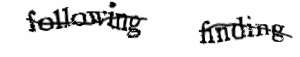
\includegraphics[width=\linewidth]{recaptcha-words}

      \smallskip
      \raggedright\small
      \lead{2007.} Два слова из отсканированных книг. Одно система знает --- по нему проверяют,
      что вы человек. Второе не смогла прочитать программа --- его читаете вы.
    \end{column}
    \begin{column}{0.47\textwidth}
      \centering
      
\includegraphics[width=0.75\linewidth]{recaptcha-house}

      \smallskip
      \begin{tikzpicture}[x=0.55cm,y=0.55cm]
        \foreach \i in {0,1,2} \foreach \j in {0,1,2}
          \fill[acLight] (\i*1.1,-\j*1.1) rectangle ++(1,-1);
        \foreach \i/\j in {0/0,2/1,1/2} {
          \fill[acDark] (\i*1.1+0.38,-\j*1.1-0.12) rectangle ++(0.24,-0.62);
          \fill[red!70] (\i*1.1+0.5,-\j*1.1-0.24) circle (0.07);
          \fill[yellow!80!orange] (\i*1.1+0.5,-\j*1.1-0.43) circle (0.07);
          \fill[green!60!black] (\i*1.1+0.5,-\j*1.1-0.62) circle (0.07);
        }
        \node[chart label,anchor=west,text=acText,align=left] at (3.5,-1.6) {Выберите\\все светофоры};
      \end{tikzpicture}

      \smallskip
      \raggedright\small
      \lead{Позже.} Номера домов с Google Street View, затем светофоры, машины и переходы ---
      разметка для карт и беспилотников.
    \end{column}
  \end{columns}

\end{frame}

\begin{frame}[c]{Волк или хаски?}
  \small Учим классификатор отличать волков от хаски. Вот часть обучающей выборки:

  \medskip
  \centering
  \begin{minipage}[t]{0.235\linewidth}\centering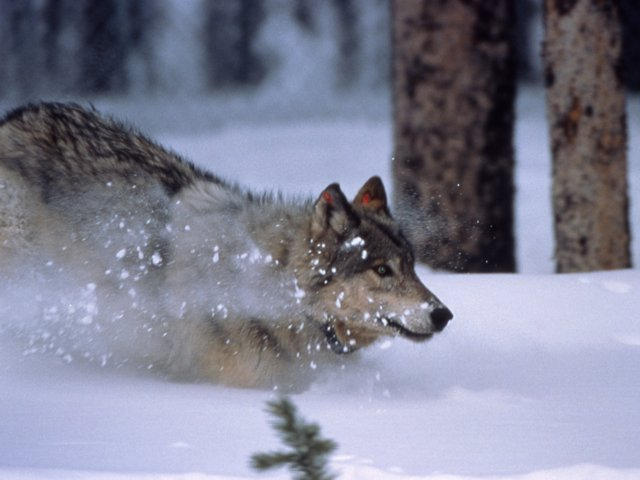
\includegraphics[width=\linewidth]{wolf-snow-1}\\[-1pt]{\scriptsize\color{acGray}волк\par}\end{minipage}\hfill
  \begin{minipage}[t]{0.235\linewidth}\centering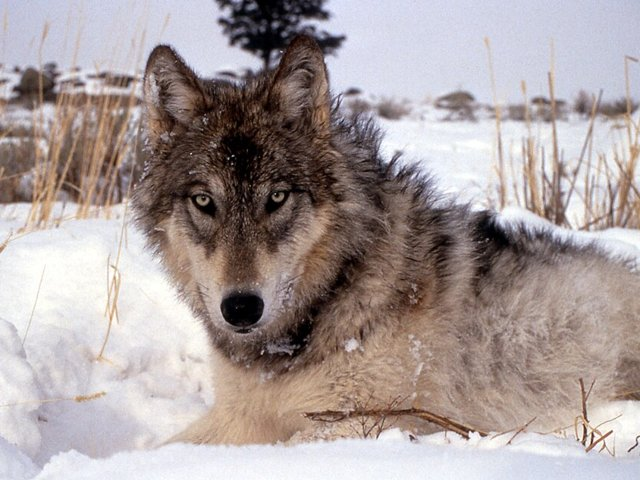
\includegraphics[width=\linewidth]{wolf-snow-2}\\[-1pt]{\scriptsize\color{acGray}волк\par}\end{minipage}\hfill
  \begin{minipage}[t]{0.235\linewidth}\centering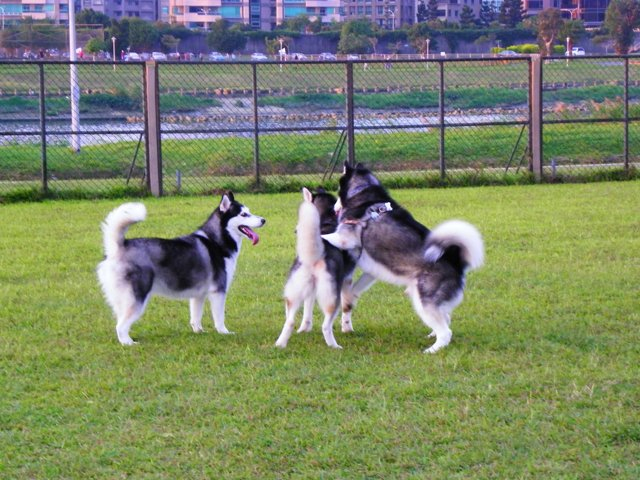
\includegraphics[width=\linewidth]{husky-grass-1}\\[-1pt]{\scriptsize\color{acGray}хаски\par}\end{minipage}\hfill
  \begin{minipage}[t]{0.235\linewidth}\centering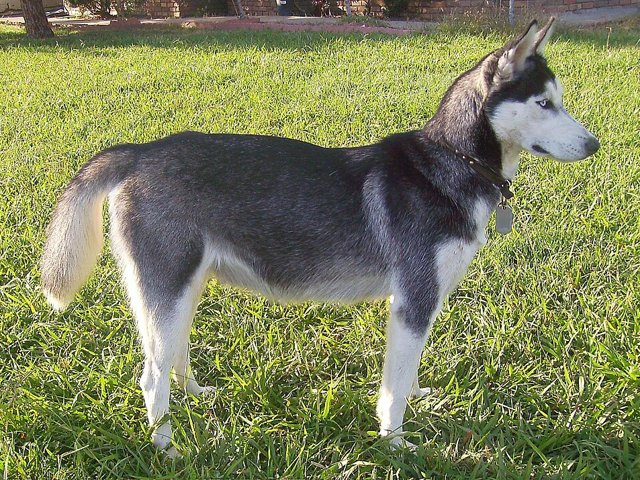
\includegraphics[width=\linewidth]{husky-grass-2}\\[-1pt]{\scriptsize\color{acGray}хаски\par}\end{minipage}

  \medskip
  \raggedright
  \lead{Вопрос.} Точность на отложенной выборке из таких же фото хорошая. Что может пойти не так?

\end{frame}

\begin{frame}[c]{Волк или хаски: ответ}
  \begin{columns}[T]
    \begin{column}{0.40\textwidth}
      \centering
      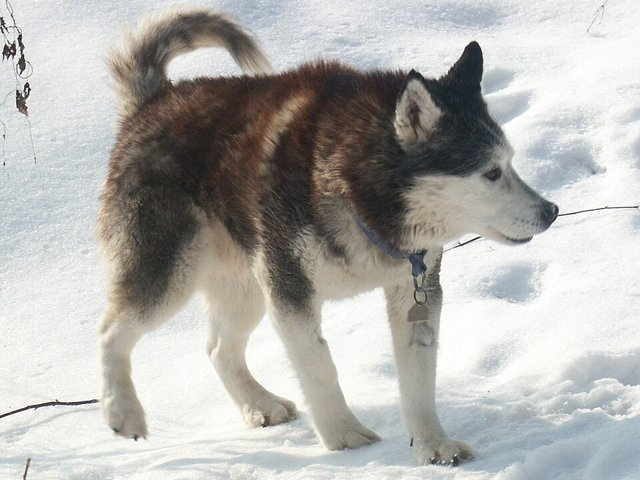
\includegraphics[width=\linewidth]{husky-snow}\\[2pt]
      {\small\color{acOrange}\bfseries Ответ модели: волк\par}
    \end{column}
    \begin{column}{0.54\textwidth}
      \begin{block}{Модель смотрела на снег}
        \small
        Все волки в обучении стояли на снегу, все хаски --- на траве.
        Проще всего отличать их по фону. Хаски на снегу --- «волк».
      \end{block}
      \begin{block}{Эксперимент (2016)}
        \small
        Исследователи специально собрали такую выборку, чтобы показать: высокая точность
        ещё не значит, что модель поняла задачу.
      \end{block}
    \end{column}
  \end{columns}

  \medskip
  \lead{Модель выучит любую закономерность, которая помогает на train,}
  даже если она случайна. Такие проблемы надо ловить при сборе данных.

\end{frame}

\begin{frame}[c]{Задание: собираем датасет листьев}
  \lead{Обсудим вместе.} Хотим, чтобы модель по фото листа определяла дерево.

  \medskip
  \begin{numrows}
    1 & Какие классы? Сколько фото на класс нужно минимум?\\
    2 & Фон, свет, ракурс: одинаковые или разные? Что будет в каждом случае?\\
    3 & Как называть файлы и где хранить ответ (породу)?\\
    4 & Если один лист сфотографирован 5 раз, можно ли эти фото раскидать в train и test?\\
    5 & Как проверить, что другой человек разметил так же?\\
  \end{numrows}
\end{frame}

\begin{frame}[c]{Ответы: правила сбора}
  \begin{columns}[T]
    \begin{column}{0.47\textwidth}
      \begin{block}{Разнообразие}
        \small
        Разные фоны, освещение и телефоны внутри \textbf{каждого} класса.
        Если все клёны сняты на асфальте, а все дубы на траве, модель выучит асфальт.
      \end{block}
      \begin{block}{Баланс}
        \small
        Примерно одинаковое число фото на класс, иначе accuracy обманет.
      \end{block}
    \end{column}
    \begin{column}{0.47\textwidth}
      \begin{block}{Утечка}
        \small
        Фото одного листа --- одна группа. Группа целиком идёт либо в train, либо в test.
        Иначе тест проверяет память, а не умение обобщать.
      \end{block}
      \begin{block}{Единый формат}
        \small
        Инструкция для всех: имя файла, папка класса, таблица с метаданными.
        Тогда датасеты всех учеников можно склеить в один.
      \end{block}
    \end{column}
  \end{columns}
\end{frame}

\section{Жизнь модели}

\begin{frame}[c]{Путь модели: от данных до инференса}
  \centering
  \begin{tikzpicture}[node distance=0.45cm]
    \node[flow box,fill=acDark] (data) {Данные};
    \node[flow box,fill=acDark,right=of data] (split) {Разбиение};
    \node[flow box,fill=acMid,right=of split] (train) {Обучение};
    \node[flow box,fill=acMid,right=of train] (val) {Валидация};
    \node[flow box,fill=acOrange,right=of val] (test) {Тест};
    \node[flow box,fill=acDark,right=of test] (inf) {Инференс};
    \foreach \a/\b in {data/split,split/train,train/val,val/test,test/inf}
      \draw[flow arrow] (\a) -- (\b);
    \draw[flow arrow] (val.north) to[out=135,in=45] node[chart label,above] {меняем гиперпараметры} (train.north);
  \end{tikzpicture}

  \medskip
  \begin{columns}[T]
    \begin{column}{0.31\textwidth}
      \begin{block}{train}
        \small
        Подбираем параметры $w$: минимизируем ошибку градиентным спуском.
        Здесь же считаем среднее и std для нормализации.
      \end{block}
    \end{column}
    \begin{column}{0.31\textwidth}
      \begin{block}{validation}
        \small
        Выбираем гиперпараметры: $k$ в KNN, шаг $\eta$, число итераций.
        Смотрим сколько угодно раз.
      \end{block}
    \end{column}
    \begin{column}{0.31\textwidth}
      \begin{block}{test}
        \small
        Один раз в конце, чтобы честно сообщить качество.
        Подсмотрели и поменяли модель --- тест испорчен.
      \end{block}
    \end{column}
  \end{columns}
\end{frame}

\begin{frame}[c]{Инференс: модель в работе}
  \begin{columns}[T]
    \begin{column}{0.47\textwidth}
      \begin{block}{Что происходит}
        \small
        Приходит новый объект без ответа. Модель только считает $\hat y = f(x; w)$.
        Параметры $w$ заморожены, градиенты не считаем.
      \end{block}
      \begin{block}{Та же предобработка}
        \small
        Нормализуем новый объект средним и std \textbf{с train}, а не по новым данным.
      \end{block}
    \end{column}
    \begin{column}{0.47\textwidth}
      \begin{block}{Что важно}
        \small
        \begin{itemize}
          \item скорость: ответ нужен за миллисекунды
          \item память: модель должна влезть в телефон или сервер
          \item стоимость: инференс идёт миллионы раз, обучение --- один
        \end{itemize}
      \end{block}
    \end{column}
  \end{columns}
\end{frame}

\begin{frame}[c]{Кросс-валидация}
  \begin{columns}[T]
    \begin{column}{0.52\textwidth}
      \centering
      \begin{tikzpicture}[x=0.95cm,y=0.48cm]
        \foreach \r/\acc in {1/0{,}82,2/0{,}86,3/0{,}84,4/0{,}88,5/0{,}85} {
          \foreach \c in {1,...,5} {
            \ifnum\c=\r
              \fill[acOrange] (\c-1,-\r) rectangle ++(0.92,0.8);
            \else
              \fill[acLight] (\c-1,-\r) rectangle ++(0.92,0.8);
            \fi
          }
          \node[chart label,anchor=east] at (-0.1,-\r+0.4) {\r};
          \node[chart label,anchor=west,text=acText] at (5,-\r+0.4) {\acc};
        }
        \node[chart label,anchor=south] at (2.46,-0.1) {выборка, разбитая на 5 частей};
        \node[chart label,anchor=south,text=acText] at (5.5,-0.1) {acc};
      \end{tikzpicture}

      \smallskip
      {\footnotesize\color{acGray}\textcolor{acOrange}{$\blacksquare$}~валидация \quad
      \textcolor{acLight!80!black}{$\blacksquare$}~обучение\par}
    \end{column}
    \begin{column}{0.44\textwidth}
      \begin{block}{$k$-fold}
        \small
        Делим train на $k$ частей. $k$ раз обучаем модель заново,
        каждый раз проверяем на новой части.
      \end{block}
      \begin{block}{Что получаем}
        \small
        Не одно число, а пять: \\
        \centerline{$\text{acc} = 0{,}85 \pm 0{,}02$}
        Видно и среднее качество, и насколько оно скачет.
      \end{block}
    \end{column}
  \end{columns}

  \medskip
  {\footnotesize\color{acGray}Минус: обучаем модель $k$ раз. Для маленьких данных это почти всегда того стоит.\par}
\end{frame}

\begin{frame}[c]{Модель B лучше модели A?}
  \lead{Вопрос.} На тесте модель A дала accuracy $0{,}85$, а модель B --- $0{,}86$. Берём B?

  \medskip
  \begin{columns}[T]
    \begin{column}{0.47\textwidth}
      \begin{block}{Тест из 100 объектов}
        \small
        Разница --- \textbf{один} объект. Погрешность accuracy примерно
        \[\pm 2\sqrt{\tfrac{p(1-p)}{n}} = \pm 2\sqrt{\tfrac{0{,}85\cdot0{,}15}{100}} \approx \pm 0{,}07.\]
        Разница $0{,}01$ тонет в шуме.
      \end{block}
    \end{column}
    \begin{column}{0.47\textwidth}
      \begin{block}{Тест из 10\,000 объектов}
        \small
        Та же формула даёт погрешность около $\pm 0{,}007$.
        Разница $0{,}01$ уже похожа на настоящую.
      \end{block}
      \begin{block}{Правило на практике}
        \small
        Если разница меньше разброса между фолдами, не верим ей.
      \end{block}
    \end{column}
  \end{columns}

  \medskip
  {\footnotesize\color{acGray}Откуда формула: каждый объект теста --- «монетка», угаданная с вероятностью $p$.
  Доля угаданных из $n$ имеет стандартное отклонение $\sqrt{p(1-p)/n}$ (биномиальное распределение),
  а в $\pm 2$ стандартных отклонения попадает около 95\,\% случаев.\par}
\end{frame}

\begin{frame}[c]{На каком этапе это происходит?}
  \begin{numrows}
    1 & Выбрать число соседей $k$ в KNN\\
    2 & Посчитать среднее и std признаков для нормализации\\
    3 & Показать пользователю рекомендации в приложении\\
    4 & Сообщить итоговую accuracy в отчёте\\
    5 & Сделать шаг градиентного спуска\\
  \end{numrows}
\end{frame}

\begin{frame}[c]{Ответы: этапы}
  \begin{numrows}
    1 & Валидация (или кросс-валидация): это гиперпараметр\\
    2 & Обучение: только по train, иначе утечка\\
    3 & Инференс\\
    4 & Тест, один раз\\
    5 & Обучение\\
  \end{numrows}
\end{frame}

\section{Производная}

\begin{frame}[c]{Таблица производных и правила}
  \begin{columns}[T]
    \begin{column}{0.40\textwidth}
      \centering
      \zebra{2}
      \begin{tabular}{cc}
        \textbf{$f(x)$} & \textbf{$f'(x)$}\\
        $c$ & $0$\\
        $x^n$ & $n\,x^{n-1}$\\
        $e^x$ & $e^x$\\
        $\ln x$ & $\dfrac1x$\\
        $\sin x$ & $\cos x$\\
        $\cos x$ & $-\sin x$\\
      \end{tabular}
    \end{column}
    \begin{column}{0.54\textwidth}
      \begin{block}{Правила}
        \small
        \begin{tabular}{@{}ll@{}}
          сумма & $(f+g)' = f' + g'$\\[3pt]
          число & $(c\,f)' = c\,f'$\\[3pt]
          произведение & $(f g)' = f' g + f g'$\\[3pt]
          \multicolumn{2}{@{}l}{\textbf{сложная функция}}\\[2pt]
          \multicolumn{2}{@{}l}{\quad$\bigl(f(g(x))\bigr)' = f'\bigl(g(x)\bigr)\cdot g'(x)$}\\
        \end{tabular}
      \end{block}
      \begin{block}{Цепное правило словами}
        \small
        Производная внешней функции, внутренность не трогаем, умножить на производную
        внутренней.
      \end{block}
    \end{column}
  \end{columns}
\end{frame}

\begin{frame}[c]{Разминка: правила}
  \lead{Самостоятельно.} Найдите производные.

  \medskip
  \begin{numrows}
    1 & $f(x) = 4x^3 - 2x + 7$\\
    2 & $f(x) = 3\sin x + e^x$\\
  \end{numrows}
\end{frame}

\begin{frame}[c]{Ответы: разминка}
  \begin{numrows}
    1 & $12x^2 - 2$\\
    2 & $3\cos x + e^x$\\
  \end{numrows}
\end{frame}

\begin{frame}[c]{Цепное правило на примерах}
  \zebra{2}
  \begin{tabular}{lll}
    \textbf{Функция} & \textbf{Внешняя и внутренняя} & \textbf{Производная}\\
    $(3x-1)^2$ & $u^2$, \ $u = 3x-1$ & $2(3x-1)\cdot 3 = 6(3x-1)$\\
    $\sin^2 x$ & $u^2$, \ $u = \sin x$ & $2\sin x\cos x$\\
    $\ln(x^2+1)$ & $\ln u$, \ $u = x^2+1$ & $\dfrac{2x}{x^2+1}$\\
    $e^{-x^2}$ & $e^u$, \ $u = -x^2$ & $-2x\,e^{-x^2}$\\
  \end{tabular}

  \medskip
  {\footnotesize\color{acGray}Проверить себя можно численно:
  $f'(x) \approx \frac{f(x+h)-f(x-h)}{2h}$ при маленьком $h$, например $10^{-5}$.\par}
\end{frame}

\begin{frame}[c]{Самостоятельно: цепное правило}
  \begin{numrows}
    1 & $f(x) = (2x+5)^3$\\
    2 & $f(x) = x\,e^{2x}$ \quad{\footnotesize\color{acGray}(произведение и цепное правило)}\\
    $\bigstar$ & $\sigma(x) = \dfrac{1}{1 + e^{-x}}$. Покажите, что $\sigma'(x) = \sigma(x)\bigl(1 - \sigma(x)\bigr)$\\
  \end{numrows}
\end{frame}

\begin{frame}[c]{Ответы: цепное правило}
  \begin{numrows}
    1 & $3(2x+5)^2\cdot 2 = 6(2x+5)^2$\\
    2 & $e^{2x} + 2x\,e^{2x} = (1 + 2x)\,e^{2x}$\\
    $\bigstar$ & $\sigma' = \dfrac{e^{-x}}{(1+e^{-x})^2} = \dfrac{1}{1+e^{-x}}\cdot\dfrac{e^{-x}}{1+e^{-x}} = \sigma\,(1-\sigma)$\\
  \end{numrows}
\end{frame}

\begin{frame}[c]{Производная по параметру, а не по $x$}
  \lead{В ML переменная --- это параметр модели, а данные $x$, $y$ --- просто числа.}

  \medskip
  \begin{columns}[T]
    \begin{column}{0.47\textwidth}
      \begin{block}{Ошибка на одном объекте}
        \small
        \[\frac{\partial}{\partial w}(w x - y)^2 = 2(wx-y)\cdot x\]
        Внешняя функция --- квадрат, внутренняя --- $wx-y$. Её производная по $w$ равна $x$.
      \end{block}
    \end{column}
    \begin{column}{0.47\textwidth}
      \begin{block}{Два признака}
        \small
        \[\frac{\partial}{\partial w_2}(w_1 x_1 + w_2 x_2 - y)^2 = 2(w_1 x_1 + w_2 x_2 - y)\cdot x_2\]
        $w_1$ при этом считаем числом: производная по $w_2$ от $w_1 x_1$ равна нулю.
      \end{block}
    \end{column}
  \end{columns}
\end{frame}

\begin{frame}[c]{Самостоятельно: производная по параметру}
  \begin{numrows}
    1 & $L(b) = (3w + b - 7)^2$ по $b$\\
    2 & $L(w) = e^{w x}$ по $w$\\
  \end{numrows}
\end{frame}

\begin{frame}[c]{Ответы: производная по параметру}
  \begin{numrows}
    1 & $2(3w + b - 7)$\\
    2 & $x\,e^{wx}$: здесь $x$ --- число\\
  \end{numrows}
\end{frame}

\section{Градиент}

\begin{frame}[c,fragile]{Частные производные и градиент}
  \begin{columns}[T]
    \begin{column}{0.52\textwidth}
      \begin{block}{Пример}
        \small
        \[f(x, y) = x^2 + xy + 2y^2\]
        Производная по $x$: $y$ считаем числом. По $y$: $x$ считаем числом.
        \[\frac{\partial f}{\partial x} = 2x + y, \qquad \frac{\partial f}{\partial y} = x + 4y\]
        \[\nabla f = \begin{pmatrix} 2x+y\\ x+4y\end{pmatrix},\qquad
          \nabla f(1, 1) = \begin{pmatrix} 3\\ 5\end{pmatrix}\]
      \end{block}
    \end{column}
    \begin{column}{0.44\textwidth}
      \centering
      \begin{tikzpicture}[scale=0.62]
        % level lines of x^2 + xy + 2y^2 = c
        \foreach \c in {1,2.5,4,6} {
          \draw[level line,rotate=-22.5] (0,0) ellipse ({sqrt(\c/0.793)} and {sqrt(\c/2.207)});
        }
        \fill[acDark] (1,1) circle (2.2pt);
        \draw[-{Stealth[length=2.2mm]},acOrange,line width=1.2pt] (1,1) -- ++(0.36,0.6)
          node[chart label,anchor=south,text=acOrange] {$\nabla f$};
        \draw[-{Stealth[length=2.2mm]},acDark,line width=1.2pt] (1,1) -- ++(-0.36,-0.6)
          node[chart label,anchor=north east,text=acDark] {$-\nabla f$};
        \fill[acDark] (0,0) circle (1.4pt);
      \end{tikzpicture}

      \smallskip
      \footnotesize\color{acGray}Линии уровня: $f$ одинакова вдоль каждой.
      Градиент перпендикулярен им и смотрит в сторону роста.
    \end{column}
  \end{columns}

  \medskip
  {\footnotesize\color{acGray}\href{https://www.geogebra.org/3d?command=f(x,y)=x^2%2Bx*y%2B2*y^2%3BSetFilling(f,0.35)%3BB=Point(f)%3BSetCoords(B,1,1,4)%3BA=(x(B),y(B),0)%3Bg=Vector(B,B%2B(2x(B)%2By(B),x(B)%2B4y(B),0))%3BSetColor(g,%22Orange%22)%3BSetLineThickness(g,10)}{\textcolor{acMid}{Откройте в GeoGebra 3D}}:
  точку $B$ можно двигать по поверхности, оранжевый вектор --- $\nabla f$ в этой точке.\par}
\end{frame}

\begin{frame}[c]{Градиент и сдвиг параметров}
  \begin{columns}[T]
    \begin{column}{0.47\textwidth}
      \begin{block}{Определение}
        \small
        Градиент --- вектор из всех частных производных:
        \[\nabla f(w) = \Bigl(\frac{\partial f}{\partial w_1}, \dots, \frac{\partial f}{\partial w_k}\Bigr)\]
      \end{block}
      \begin{block}{Сдвиг $h$}
        \small
        На сколько меняем каждый параметр: $w \to w + h$.
        Пример: $(1, 1) + (-0{,}15;\ -0{,}25) = (0{,}85;\ 0{,}75)$.
      \end{block}
    \end{column}
    \begin{column}{0.47\textwidth}
      \begin{block}{Линейное приближение}
        \small
        Если $h$ маленький, функция рядом почти плоская:
        \[f(w + h) \approx f(w) + \nabla f(w)\cdot h\]
        Справа скалярное произведение:
        \[\nabla f\cdot h = \frac{\partial f}{\partial w_1} h_1 + \dots + \frac{\partial f}{\partial w_k} h_k\]
        Каждый параметр сдвинули --- функция изменилась примерно на «наклон $\times$ сдвиг».
      \end{block}
    \end{column}
  \end{columns}
\end{frame}

\begin{frame}[c]{Почему шаг против градиента уменьшает функцию}
  \begin{columns}[T]
    \begin{column}{0.47\textwidth}
      \begin{block}{Куда шагнуть}
        \small
        Изменение функции:
        \[\nabla f\cdot h = \lVert\nabla f\rVert\,\lVert h\rVert\cos\varphi\]
        При шаге фиксированной длины оно самое отрицательное при $\cos\varphi = -1$,
        то есть когда $h$ смотрит \textbf{против} градиента.
      \end{block}
    \end{column}
    \begin{column}{0.47\textwidth}
      \begin{block}{Шаг ГД}
        \small
        Берём $h = -\eta\nabla f$:
        \[f(w - \eta\nabla f) \approx f(w) - \eta\lVert\nabla f\rVert^2 < f(w)\]
      \end{block}
      \begin{block}{Проверим на числах}
        \small
        $f = x^2 + xy + 2y^2$, $w = (1, 1)$, $f = 4$, $\nabla f = (3, 5)$, $\eta = 0{,}05$.
        Прогноз $4 - 0{,}05\cdot 34 = 2{,}3$, на деле $f(0{,}85;\ 0{,}75) \approx 2{,}49$.
      \end{block}
    \end{column}
  \end{columns}
\end{frame}

\begin{frame}[c]{Много параметров: линейная регрессия}
  \small
  Объект --- $k$ признаков, модель $\hat y_i = w_1 x_{i1} + \dots + w_k x_{ik}$. Ошибка
  $\;\mathrm{err}_i = \hat y_i - y_i$.

  \medskip
  \begin{columns}[T]
    \begin{column}{0.47\textwidth}
      \begin{block}{Шаг 1. Один объект}
        \small
        Цепное правило:
        \[\frac{\partial}{\partial w_j}\,\mathrm{err}_i^2 = 2\,\mathrm{err}_i\cdot x_{ij}\]
      \end{block}
    \end{column}
    \begin{column}{0.47\textwidth}
      \begin{block}{Шаг 2. Среднее по объектам}
        \small
        Производная суммы --- сумма производных:
        \[g_j = \frac{2}{n}\sum_{i=1}^{n} x_{ij}\,\mathrm{err}_i\]
      \end{block}
    \end{column}
  \end{columns}

  \medskip
  \lead{Это просто цикл:} для каждого параметра $j$ пробегаем объекты и копим сумму.
  Осталось заметить, что такой цикл уже есть в numpy.
\end{frame}

\begin{frame}[c]{Шаг 3. Цикл --- это $X^\top \mathrm{err}$}
  \begin{columns}[T]
    \begin{column}{0.50\textwidth}
      \small
      3 объекта, 2 признака:
      \[X = \begin{pmatrix} 1 & 2\\ 3 & 0\\ 0 & 1\end{pmatrix},\qquad
        \mathrm{err} = \begin{pmatrix} 1\\ -1\\ 2\end{pmatrix}\]
      \textbf{Циклом:}
      \begin{align*}
        \textstyle\sum_i x_{i1}\mathrm{err}_i &= 1\cdot1 + 3\cdot(-1) + 0\cdot2 = -2\\
        \textstyle\sum_i x_{i2}\mathrm{err}_i &= 2\cdot1 + 0\cdot(-1) + 1\cdot2 = 4
      \end{align*}
    \end{column}
    \begin{column}{0.46\textwidth}
      \small
      \textbf{Матрицей:} столбец $j$ матрицы $X$ --- это строка $j$ в $X^\top$.
      \[X^\top \mathrm{err} =
        \begin{pmatrix} 1 & 3 & 0\\ 2 & 0 & 1\end{pmatrix}
        \begin{pmatrix} 1\\ -1\\ 2\end{pmatrix} =
        \begin{pmatrix} -2\\ 4\end{pmatrix}\]
      \lead{Ответы совпали.}
      \[\nabla \mathrm{MSE} = \frac{2}{n}\,X^\top (Xw - y)\]
    \end{column}
  \end{columns}
\end{frame}

\begin{frame}[c]{Правило размерностей}
  \lead{Не помните, где транспонировать? Проверьте формы.}

  \medskip
  \centering
  \zebra{2}
  \begin{tabular}{lcl}
    \textbf{Что} & \textbf{Форма} & \textbf{Смысл}\\
    $X$ & $n\times k$ & объекты $\times$ признаки\\
    $w$ & $k\times 1$ & по весу на признак\\
    $Xw - y$ & $n\times 1$ & по ошибке на объект\\
    $\nabla$ & $k\times 1$ & \textbf{как у $w$}: по числу на параметр\\
  \end{tabular}

  \medskip
  \raggedright\small
  Из $X$ ($n\times k$) и ошибок ($n\times1$) получить $k\times1$ можно только так:
  $(k\times n)\cdot(n\times 1)$, то есть $X^\top\mathrm{err}$. Если формы не сходятся --- формула неверна.

  \medskip
  \centerline{\texttt{grad = 2 / n * X.T @ (X @ w - y)}}
\end{frame}

\section{Градиентный спуск}

\begin{frame}[c,fragile]{Градиентный спуск для $k$ параметров}
  \begin{columns}[T]
    \begin{column}{0.47\textwidth}
      \begin{block}{Алгоритм}
        \small
        \begin{enumerate}\setlength\itemsep{0.25em}
          \item Начальное $w$: нули или случайные числа.
          \item Считаем $\nabla L(w)$ по всем объектам.
          \item Обновляем \textbf{все} параметры сразу:
            \(w \leftarrow w - \eta\,\nabla L(w)\)
          \item Повторяем, пока $\lVert\nabla L\rVert$ не станет маленьким
            или не кончится лимит итераций.
        \end{enumerate}
      \end{block}
    \end{column}
    \begin{column}{0.47\textwidth}
      \begin{block}{Код}
        \small
\begin{semiverbatim}
w = np.zeros(k)
for step in range(1000):
    err = X @ w - y
    grad = 2 / n * X.T @ err
    if np.linalg.norm(grad) < eps:
        break
    w = w - lr * grad
\end{semiverbatim}
      \end{block}
    \end{column}
  \end{columns}

  \medskip
  {\footnotesize\color{acGray}Если функция не парабола, минимумов может быть несколько:
  куда придём, зависит от стартовой точки.\par}
\end{frame}

\begin{frame}[c]{Стохастический градиентный спуск (SGD)}
  \begin{columns}[T]
    \begin{column}{0.47\textwidth}
      \begin{block}{Проблема}
        \small
        Шаг ГД --- проход по \textbf{всем} $n$ объектам. При $n = 10^7$ это долго.
      \end{block}
      \begin{block}{Идея}
        \small
        Градиент по случайному батчу из $B$ объектов, например $B = 64$:
        \[\nabla L \approx \frac{2}{B}\,X_B^\top (X_B w - y_B)\]
      \end{block}
    \end{column}
    \begin{column}{0.47\textwidth}
      \centering
      \begin{tikzpicture}[scale=0.85]
        \foreach \c in {0.4,1.2,2.4,4} {
          \draw[level line] (0,0) ellipse ({sqrt(\c)} and {0.6*sqrt(\c)});
        }
        \draw[gd path,draw=acDark] (-1.9,0.6) -- (-1.15,0.36) -- (-0.6,0.19) -- (-0.25,0.08) -- (-0.05,0.02);
        \draw[gd path] (-1.9,0.6) -- (-1.5,0.15) -- (-1.25,0.62) -- (-0.8,0.05) -- (-0.7,0.4)
          -- (-0.3,-0.1) -- (-0.15,0.22) -- (0.05,-0.05);
        \fill[acDark] (0,0) circle (1.6pt);
        \node[chart label,anchor=north] at (0,-1.35) {\textcolor{acDark}{---}~ГД \quad \textcolor{acOrange}{---}~SGD};
      \end{tikzpicture}

      \smallskip
      \raggedright\small
      Шаги SGD шумные, но каждый в $n/B$ раз дешевле.
      Проход по всем данным батчами --- \textbf{эпоха}.
      Так учат почти все нейросети.
    \end{column}
  \end{columns}
\end{frame}

\begin{frame}[c]{Зачем нормализовать признаки}
  \small
  200 квартир: площадь 30--120\,м\textsuperscript{2}, комнат 1--4. Цена $\approx 0{,}05\cdot\text{площадь} + 0{,}8\cdot\text{комнаты}$.

  \medskip
  \begin{columns}[T]
    \begin{column}{0.47\textwidth}
      \begin{block}{Без нормализации}
        \small
        Первый градиент из $w = 0$:
        \[\nabla L = \begin{pmatrix} -936\\ -30\end{pmatrix}\]
        По площади в 30 раз больше: значения признака больше, а в $g_j$ стоит множитель $x_{ij}$.
      \end{block}
    \end{column}
    \begin{column}{0.47\textwidth}
      \begin{block}{Шаг один на всех}
        \small
        Шаг ограничен «площадью». При таком шаге вес комнат еле двигается.
        \smallskip
        \zebra{2}\small
        \begin{tabular}{lr}
          \textbf{Шаг $\eta$} & \textbf{Итераций}\\
          $10^{-3}$ & расходится\\
          $3\cdot10^{-4}$ & расходится\\
          $10^{-4}$ & 21\,404\\
        \end{tabular}
      \end{block}
    \end{column}
  \end{columns}
\end{frame}

\begin{frame}[c]{Овраг и круг}
  \begin{columns}[T]
    \begin{column}{0.47\textwidth}
      \centering
      \begin{tikzpicture}[scale=0.78]
        \useasboundingbox (-3.7,-1.6) rectangle (3.7,1.6);
        \foreach \c in {0.8,2.5,6,12.8} {
          \draw[level line] (0,0) ellipse ({sqrt(\c)} and {sqrt(\c/20)});
        }
        \draw[gd path] plot coordinates {(-2.60,0.55) (-2.37,-0.44) (-2.15,0.35) (-1.96,-0.28)
          (-1.78,0.23) (-1.62,-0.18) (-1.48,0.14) (-1.34,-0.12) (-1.22,0.09) (-1.11,-0.07)
          (-1.01,0.06) (-0.92,-0.05) (-0.84,0.04)};
        \fill[acDark] (0,0) circle (1.6pt);
      \end{tikzpicture}

      \smallskip
      \lead{Без нормализации}\\
      \small Линии уровня вытянуты. ГД скачет поперёк оврага и медленно ползёт вдоль.
    \end{column}
    \begin{column}{0.47\textwidth}
      \centering
      \begin{tikzpicture}[scale=0.78]
        \useasboundingbox (-3.7,-1.6) rectangle (3.7,1.6);
        \foreach \r in {0.5,1,1.5} {
          \draw[level line] (0,0) circle (\r);
        }
        \draw[gd path] plot coordinates {(-1.20,0.90) (-0.48,0.36) (-0.19,0.14) (-0.08,0.06) (-0.03,0.02)};
        \fill[acDark] (0,0) circle (1.6pt);
      \end{tikzpicture}

      \smallskip
      \lead{После стандартизации}\\
      \small Градиенты одного порядка, можно взять большой шаг:
      $\eta = 0{,}3$ --- \textbf{11} итераций вместо 21\,404.
    \end{column}
  \end{columns}

  \medskip
  {\footnotesize\color{acGray}Стандартизация: $x' = (x - \text{среднее})/\text{std}$.
  Среднее и std считаем только на train.\par}
\end{frame}

\begin{frame}[c]{Слишком большой шаг}
  \small $L(w_1, w_2) = w_1^2 + 3w_2^2$, старт в одной и той же точке. Листайте: каждый клик --- один шаг ГД.
  Пунктир --- часть шага, скрытая за передней стенкой чаши.

  \smallskip
  \begin{columns}[T]
    \begin{column}{0.49\textwidth}
      \centering
      \begin{tikzpicture}
        \begin{axis}[width=6.2cm,height=4.9cm,view={35}{50},
            xmin=-2,xmax=2,ymin=-1.6,ymax=1.6,zmin=0,zmax=12,
            xlabel={$w_1$},ylabel={$w_2$},zlabel={$L$},
            ticks=none,axis lines=box,axis line style={draw=acGray!50},
            label style={font=\scriptsize,text=acGray},
            colormap={ac}{color=(acLight) color=(acMid!70)},
            title={\small $\eta = 0{,}1$: спускаемся},title style={text=acDark}]
          \addplot3[surf,shader=faceted interp,draw=white,line width=0.2pt,opacity=0.75,
            domain=-2:2,y domain=-1.6:1.6,samples=21,samples y=21]
            {min(x^2+3*y^2,12)};
          \only<2->{\addplot3[gd path] coordinates {(-1.600,0.800,4.480) (-1.280,0.320,1.946)};
            \addplot3[gd end] coordinates {(-1.280,0.320,1.946)};}
          \only<3->{\addplot3[gd path] coordinates {(-1.280,0.320,1.946) (-1.024,0.128,1.098)};
            \addplot3[gd end] coordinates {(-1.024,0.128,1.098)};}
          \only<4->{\addplot3[gd path] coordinates {(-1.024,0.128,1.098) (-0.819,0.051,0.679)};
            \addplot3[gd end] coordinates {(-0.819,0.051,0.679)};}
          \only<5->{\addplot3[gd path] coordinates {(-0.819,0.051,0.679) (-0.655,0.020,0.431)};
            \addplot3[gd end] coordinates {(-0.655,0.020,0.431)};}
          \only<6->{\addplot3[gd path] coordinates {(-0.655,0.020,0.431) (-0.524,0.008,0.275)};
            \addplot3[gd end] coordinates {(-0.524,0.008,0.275)};}
          \only<7->{\addplot3[gd path] coordinates {(-0.524,0.008,0.275) (-0.419,0.003,0.176)};
            \addplot3[gd end] coordinates {(-0.419,0.003,0.176)};}
          \addplot3[only marks,mark=*,mark size=1.8pt,mark options={fill=acDark,draw=acDark}] coordinates {(-1.600,0.800,4.480)};
          \addplot3[only marks,mark=x,mark size=2.5pt,acDark,thick] coordinates {(0,0,0)};
        \end{axis}
      \end{tikzpicture}
    \end{column}
    \begin{column}{0.49\textwidth}
      \centering
      \begin{tikzpicture}
        \begin{axis}[width=6.2cm,height=4.9cm,view={35}{50},
            xmin=-2,xmax=2,ymin=-1.6,ymax=1.6,zmin=0,zmax=12,
            xlabel={$w_1$},ylabel={$w_2$},zlabel={$L$},
            ticks=none,axis lines=box,axis line style={draw=acGray!50},
            label style={font=\scriptsize,text=acGray},
            colormap={ac}{color=(acLight) color=(acMid!70)},
            title={\small $\eta = 0{,}35$: перепрыгиваем},title style={text=acDark}]
          \addplot3[surf,shader=faceted interp,draw=white,line width=0.2pt,opacity=0.75,
            domain=-2:2,y domain=-1.6:1.6,samples=21,samples y=21]
            {min(x^2+3*y^2,12)};
          \only<2->{\addplot3[gd path] coordinates {(-1.600,0.800,4.480) (-0.607,-0.690,2.771)};
            \addplot3[gd path,dash pattern=on 1.6pt off 1.3pt] coordinates {(-0.607,-0.690,2.771) (-0.480,-0.880,2.554)};
            \addplot3[gd end hidden] coordinates {(-0.480,-0.880,2.554)};}
          \only<3->{\addplot3[gd path,dash pattern=on 1.6pt off 1.3pt] coordinates {(-0.480,-0.880,2.554) (-0.436,-0.640,2.590)};
            \addplot3[gd path] coordinates {(-0.436,-0.640,2.590) (-0.144,0.968,2.832)};
            \addplot3[gd end] coordinates {(-0.144,0.968,2.832)};}
          \only<4->{\addplot3[gd path] coordinates {(-0.144,0.968,2.832) (-0.061,-0.699,3.300)};
            \addplot3[gd path,dash pattern=on 1.6pt off 1.3pt] coordinates {(-0.061,-0.699,3.300) (-0.043,-1.065,3.403)};
            \addplot3[gd end hidden] coordinates {(-0.043,-1.065,3.403)};}
          \only<5->{\addplot3[gd path,dash pattern=on 1.6pt off 1.3pt] coordinates {(-0.043,-1.065,3.403) (-0.039,-0.747,3.504)};
            \addplot3[gd path] coordinates {(-0.039,-0.747,3.504) (-0.013,1.171,4.116)};
            \addplot3[gd end] coordinates {(-0.013,1.171,4.116)};}
          \only<6->{\addplot3[gd path] coordinates {(-0.013,1.171,4.116) (-0.005,-1.042,4.894)};
            \addplot3[gd path,dash pattern=on 1.6pt off 1.3pt] coordinates {(-0.005,-1.042,4.894) (-0.004,-1.288,4.980)};
            \addplot3[gd end hidden] coordinates {(-0.004,-1.288,4.980)};}
          \only<7->{\addplot3[gd path,dash pattern=on 1.6pt off 1.3pt] coordinates {(-0.004,-1.288,4.980) (-0.004,-1.085,5.058)};
            \addplot3[gd path] coordinates {(-0.004,-1.085,5.058) (-0.001,1.417,6.026)};
            \addplot3[gd end] coordinates {(-0.001,1.417,6.026)};}
          \addplot3[only marks,mark=*,mark size=1.8pt,mark options={fill=acDark,draw=acDark}] coordinates {(-1.600,0.800,4.480)};
          \addplot3[only marks,mark=x,mark size=2.5pt,acDark,thick] coordinates {(0,0,0)};
        \end{axis}
      \end{tikzpicture}
    \end{column}
  \end{columns}

  \smallskip
  \visible<7>{\lead{Справа шаг перелетает дно оврага, и каждый раз мы оказываемся всё выше:
  ГД расходится.}}
\end{frame}

\begin{frame}[c]{Расписание шага}
  \begin{columns}[T]
    \begin{column}{0.40\textwidth}
      \begin{block}{Проблема}
        \small
        Большой шаг быстро подводит к минимуму, но дальше прыгает вокруг него.
        Маленький шаг медленный с самого начала.
      \end{block}
      \begin{block}{Решение}
        \small
        Начинаем с большого шага и уменьшаем его:
        \[\eta_t = \frac{\eta_0}{1 + t/T}\]
      \end{block}
    \end{column}
    \begin{column}{0.56\textwidth}
      \centering
      \begin{tikzpicture}[x=1.45cm,y=5.5cm]
        \foreach \v in {0,0.1,0.2,0.3,0.4} {
          \draw[draw=acRule,line width=0.4pt] (0,\v) -- (4,\v);
          \node[chart label,anchor=east] at (0,\v) {\v};
        }
        \draw[chart axis] (0,0) -- (4.05,0);
        \draw[chart axis] (0,0) -- (0,0.42);
        \foreach \t/\l in {0/0,1/100,2/200,3/300,4/400} \node[chart label,anchor=north] at (\t,0) {\l};
        \begin{scope}
          \clip (0,0) rectangle (4.05,0.42);
          \draw[acOrange,line width=1.1pt,line join=round] plot coordinates {(0.00,2.124) (0.10,0.353) (0.20,0.193) (0.30,0.196) (0.40,0.199) (0.50,0.203) (0.60,0.195) (0.70,0.198) (0.80,0.191) (0.90,0.224) (1.00,0.226) (1.10,0.201) (1.20,0.194) (1.30,0.207) (1.40,0.195) (1.50,0.205) (1.60,0.193) (1.70,0.198) (1.80,0.190) (1.90,0.197) (2.00,0.172) (2.10,0.230) (2.20,0.175) (2.30,0.203) (2.40,0.174) (2.50,0.182) (2.60,0.207) (2.70,0.200) (2.80,0.216) (2.90,0.197) (3.00,0.178) (3.10,0.187) (3.20,0.216) (3.30,0.211) (3.40,0.222) (3.50,0.178) (3.60,0.220) (3.70,0.171) (3.80,0.169) (3.90,0.171) (3.99,0.195)};
          \draw[acDark,line width=1.1pt,line join=round] plot coordinates {(0.00,2.124) (0.10,0.426) (0.20,0.179) (0.30,0.138) (0.40,0.130) (0.50,0.126) (0.60,0.098) (0.70,0.095) (0.80,0.102) (0.90,0.105) (1.00,0.086) (1.10,0.077) (1.20,0.091) (1.30,0.087) (1.40,0.078) (1.50,0.075) (1.60,0.072) (1.70,0.072) (1.80,0.066) (1.90,0.071) (2.00,0.065) (2.10,0.067) (2.20,0.066) (2.30,0.073) (2.40,0.062) (2.50,0.062) (2.60,0.063) (2.70,0.066) (2.80,0.063) (2.90,0.067) (3.00,0.063) (3.10,0.061) (3.20,0.065) (3.30,0.066) (3.40,0.069) (3.50,0.054) (3.60,0.056) (3.70,0.053) (3.80,0.052) (3.90,0.053) (3.99,0.049)};
        \end{scope}
        \node[chart label,anchor=north] at (2,-0.06) {шаг SGD (батч 8)};
        \node[chart label,anchor=south,rotate=90] at (-0.5,0.21) {до оптимума};
        \begin{scope}[shift={(1.6,0.39)}]
          \fill[white] (-0.08,0.025) rectangle (2.45,-0.075);
          \draw[acOrange,line width=1.1pt] (0,0) -- (0.3,0);
          \node[chart label,anchor=west,text=acText] at (0.35,0) {$\eta = 0{,}1$};
          \draw[acDark,line width=1.1pt] (0,-0.05) -- (0.3,-0.05);
          \node[chart label,anchor=west,text=acText] at (0.35,-0.05) {$\eta_t = 0{,}1/(1 + t/30)$};
        \end{scope}
      \end{tikzpicture}

      \smallskip
      \raggedright\footnotesize\color{acGray}Линейная регрессия на синтетике, 1000 объектов,
      среднее по 20 запускам. С постоянным шагом застреваем около $0{,}2$,
      с убывающим доходим до $0{,}05$. Другие расписания: делить шаг пополам каждые $T$ шагов,
      умножать на $\gamma < 1$ на каждом шаге.
    \end{column}
  \end{columns}
\end{frame}

\section{Итоги}

\begin{frame}[c]{Проверь себя}
  \begin{numrows}
    1 & Почему фото одного листа нельзя раскидать по train и test?\\
    2 & Кросс-валидация дала $0{,}84 \pm 0{,}03$ и $0{,}85 \pm 0{,}03$. Какая модель лучше?\\
    3 & $X$ имеет форму $500\times 4$. Какой формы $\nabla L$?\\
    4 & Чем шаг SGD отличается от шага ГД?\\
    5 & ГД расходится уже при маленьком шаге. Что проверить первым делом?\\
  \end{numrows}
\end{frame}

\begin{frame}[c]{Ответы}
  \begin{numrows}
    1 & Тест будет проверять память, а не обобщение: утечка\\
    2 & Сказать нельзя: разница меньше разброса\\
    3 & $4\times1$, как у $w$\\
    4 & Градиент по случайному батчу, а не по всем объектам\\
    5 & Масштаб признаков и формулу градиента\\
  \end{numrows}
\end{frame}

\begin{frame}[c]{На практике: восстановление коэффициентов}
  \small
  Даны точки $(x, f(x))$, где
  \[f(x) = \bigl((a+\varepsilon_a)\sin x + (b+\varepsilon_b)\ln x\bigr)^2 + (c+\varepsilon_c)\,x^2,
    \qquad \varepsilon \in [-0{,}001;\ 0{,}001].\]
  Нужно найти $a$, $b$, $c$ с точностью $10^{-2}$.

  \medskip
  \begin{columns}[T]
    \begin{column}{0.47\textwidth}
      \begin{block}{Подумайте}
        \small
        \begin{itemize}
          \item Что здесь данные, а что параметры?
          \item Чему равна $\partial f/\partial a$? А $\partial f/\partial c$?
        \end{itemize}
      \end{block}
    \end{column}
    \begin{column}{0.47\textwidth}
      \visible<2>{%
      \begin{block}{Подсказка}
        \small
        $\sin x$, $\ln x$, $x^2$ не зависят от $a$, $b$, $c$ ---
        это просто столбцы признаков:

        \smallskip
        \centering\footnotesize
        \zebra{2}\footnotesize
        \begin{tabular}{rrrr}
          $x$ & $\sin x$ & $\ln x$ & $x^2$\\
          $0{,}5$ & $0{,}479$ & $-0{,}693$ & $0{,}25$ \\
          $1$ & $0{,}841$ & $0{,}000$ & $1$ \\
          $2$ & $0{,}909$ & $0{,}693$ & $4$\\
        \end{tabular}
      \end{block}}
    \end{column}
  \end{columns}

  \smallskip
  {\footnotesize\color{acGray}Задача: \url{https://coderun.yandex.ru/problem/coefficients-restoration}\par}
\end{frame}

\section{Extra: матричное дифференцирование}

\begin{frame}[c]{Что такое производная по вектору и по матрице}
  \small Правило одно: \lead{производная --- это таблица частных производных, по одной на каждую пару
  «что меняется --- по чему меняем».}

  \medskip
  \zebra{2}\small\setlength{\tabcolsep}{4pt}
  \begin{tabular}{llll}
    \textbf{Что по чему} & \textbf{Результат} & \textbf{Форма} & \textbf{Пример}\\
    число по вектору $w$ & градиент: $(\nabla f)_j = \partial f/\partial w_j$ & как $w$ & $w_1^2 + 3w_2 \ \to\ (2w_1;\ 3)$\\
    число по матрице $W$ & элемент $(i,j)$: $\partial f/\partial W_{ij}$ & как $W$ & веса слоя нейросети\\
    вектор $g$ по вектору $w$ & матрица Якоби: $J_{ij} = \partial g_i/\partial w_j$ & $m\times k$ & $Xw \ \to\ J = X$\\
  \end{tabular}

  \medskip
  \raggedright
  Смысл везде тот же, что у обычной производной: при маленьком сдвиге $h$
  \[f(w + h) \approx f(w) + \nabla f(w)^\top h, \qquad g(w + h) \approx g(w) + J\,h.\]
\end{frame}

\begin{frame}[c]{Цепное правило для векторов}
  \begin{columns}[T]
    \begin{column}{0.47\textwidth}
      \begin{block}{Правило}
        \small
        Если $u = g(w)$, а $L = f(u)$ --- число, то
        \[\nabla_w L = J^\top\,\nabla_u f,\]
        где $J$ --- матрица Якоби внутренней функции $g$.
        Как в школе: производная внешней, умноженная на производную внутренней.
      \end{block}
    \end{column}
    \begin{column}{0.47\textwidth}
      \begin{block}{Пример: MSE}
        \small
        $L = \lVert u\rVert^2$, \ $u = Xw - y$.
        \begin{itemize}
          \item внешняя: $\nabla_u \lVert u\rVert^2 = 2u$
          \item внутренняя: $J = X$
        \end{itemize}
        \[\nabla_w L = X^\top\cdot 2u = 2X^\top(Xw - y)\]
      \end{block}
    \end{column}
  \end{columns}

  \medskip
  \lead{Вот откуда берётся $X^\top$:} транспонированная матрица Якоби. Формы тоже сходятся:
  $(k\times n)\cdot(n\times 1) = k\times 1$.
\end{frame}

\begin{frame}[c]{Матричные производные: шпаргалка}
  \lead{Те же правила, что в школе, только для векторов.} Здесь $w$, $a$ --- векторы длины $k$.

  \medskip
  \centering
  \zebra{2}\small\setlength{\tabcolsep}{5pt}
  \begin{tabular}{lll}
    \textbf{Одно число} & \textbf{Вектор} & \textbf{Почему}\\
    $(a w)' = a$ & $\nabla_w\,(a^\top w) = a$ & $a_1 w_1 + \dots + a_k w_k$ по $w_j$: $a_j$\\
    $(w^2)' = 2w$ & $\nabla_w\,(w^\top w) = 2w$ & $w_1^2 + \dots + w_k^2$ по $w_j$: $2w_j$\\
    $(a w^2)' = 2aw$ & $\nabla_w\,(w^\top A w) = 2Aw$ & если $A = A^\top$\\
    $\bigl((xw - y)^2\bigr)' = 2x(xw-y)$ & $\nabla_w\lVert Xw - y\rVert^2 = 2X^\top(Xw - y)$ & цепное правило\\
  \end{tabular}

  \medskip
  \raggedright\small
  В последней строке: внешняя функция --- $\lVert u\rVert^2 = u^\top u$, внутренняя --- $u = Xw - y$.
  Множитель $x$ из одномерного случая превращается в $X^\top$.
\end{frame}

\begin{frame}[c]{Градиент MSE в одну строку}
  \begin{columns}[T]
    \begin{column}{0.52\textwidth}
      \begin{block}{Раскроем квадрат}
        \small
        \[\lVert Xw - y\rVert^2 = w^\top X^\top X\, w \;-\; 2\,y^\top X w \;+\; y^\top y\]
        По шпаргалке, слагаемое за слагаемым:
        \begin{itemize}
          \item $w^\top (X^\top X)\, w$ \ $\to$ \ $2X^\top X w$ \ {\footnotesize\color{acGray}($X^\top X$ симметричная)}
          \item $-2\,(X^\top y)^\top w$ \ $\to$ \ $-2X^\top y$
          \item $y^\top y$ \ $\to$ \ $0$: не зависит от $w$
        \end{itemize}
        \[\nabla_w \mathrm{MSE} = \frac1n\bigl(2X^\top X w - 2X^\top y\bigr) = \frac2n X^\top(Xw - y)\]
      \end{block}
    \end{column}
    \begin{column}{0.44\textwidth}
      \begin{block}{Сверим}
        \small
        Тот же ответ, что мы получили циклом по объектам. Два способа --- одна формула.
      \end{block}
      \begin{block}{Попробуйте}
        \small
        $f(w) = w^\top w + a^\top w$, где $a = (1;\ -2)$. Найдите $\nabla f$ и точку, где он равен нулю.

        \smallskip
        \visible<2>{\textbf{Ответ:} $\nabla f = 2w + a$, ноль при $w = -a/2 = (-0{,}5;\ 1)$.}
      \end{block}
    \end{column}
  \end{columns}
\end{frame}

\begin{frame}[c]{Несколько слоёв: цепное правило по цепочке}
  \small Маленькая нейросеть: $\hat y = w_2\,\sigma(w_1 x)$, ошибка $L = (\hat y - y)^2$.
  Каждый слой --- одна простая функция.

  \medskip
  \centering
  \begin{tikzpicture}[
      val/.style={circle,draw=acMid,fill=acLight,minimum size=0.75cm,inner sep=0pt,font=\small},
      op/.style={rectangle,rounded corners=2pt,fill=acDark,text=white,font=\scriptsize\bfseries,
        minimum height=0.55cm,inner sep=3pt},
      fwd/.style={-{Stealth[length=2mm]},line width=0.9pt,color=acGray},
      bwd/.style={-{Stealth[length=2mm]},line width=0.9pt,color=acOrange}]
    \node[val] (x) at (0,0) {$x$};
    \node[op] (o1) at (1.35,0) {$\times w_1$};
    \node[val] (z) at (2.7,0) {$z$};
    \node[op] (o2) at (4.05,0) {$\sigma$};
    \node[val] (h) at (5.4,0) {$h$};
    \node[op] (o3) at (6.75,0) {$\times w_2$};
    \node[val] (yh) at (8.1,0) {$\hat y$};
    \node[op] (o4) at (9.6,0) {$(\cdot - y)^2$};
    \node[val,draw=acOrange] (L) at (11.1,0) {$L$};
    \foreach \a/\b in {x/o1,o1/z,z/o2,o2/h,h/o3,o3/yh,yh/o4,o4/L} \draw[fwd] (\a) -- (\b);
    \node[chart label,anchor=south] at (5.55,0.45) {прямой проход: считаем значения};
    \draw[bwd] (L.south) to[out=-150,in=-30] node[chart label,below,text=acOrange] {$2(\hat y - y)$} (yh.south);
    \draw[bwd] (yh.south) to[out=-150,in=-30] node[chart label,below,text=acOrange] {$w_2$} (h.south);
    \draw[bwd] (h.south) to[out=-150,in=-30] node[chart label,below,text=acOrange] {$\sigma'(z)$} (z.south);
    \draw[bwd] (z.south) to[out=-150,in=-30] node[chart label,below,text=acOrange] {$x$} (x.south);
    \node[chart label,anchor=north,text=acOrange] at (5.55,-1.45) {обратный проход: перемножаем локальные производные};
  \end{tikzpicture}

  \medskip
  \[\frac{\partial L}{\partial w_1} = \underbrace{2(\hat y - y)}_{\partial L/\partial \hat y}\cdot
    \underbrace{w_2}_{\partial \hat y/\partial h}\cdot
    \underbrace{\sigma'(z)}_{\partial h/\partial z}\cdot
    \underbrace{x}_{\partial z/\partial w_1}\]

  \raggedright\small
  \lead{Это и есть backpropagation.} Каждый слой знает только свою производную, а произведения
  справа налево переиспользуются для всех слоёв.
\end{frame}

\begin{frame}[c]{Backpropagation на числах}
  \small $x = 1$, $y = 1$, $w_1 = 0{,}5$, $w_2 = 2$, $\sigma$ --- сигмоида, $\sigma'(z) = \sigma(z)\bigl(1 - \sigma(z)\bigr)$.

  \medskip
  \begin{columns}[T]
    \begin{column}{0.44\textwidth}
      \begin{block}{Прямой проход}
        \small
        \begin{tabular}{@{}ll@{}}
          $z = w_1 x$ & $= 0{,}5$\\
          $h = \sigma(z)$ & $\approx 0{,}622$\\
          $\hat y = w_2 h$ & $\approx 1{,}245$\\
          $L = (\hat y - y)^2$ & $\approx 0{,}060$\\
        \end{tabular}
      \end{block}
    \end{column}
    \begin{column}{0.52\textwidth}
      \begin{block}{Обратный проход}
        \small
        \begin{tabular}{@{}ll@{}}
          $\partial L/\partial \hat y = 2(\hat y - y)$ & $\approx 0{,}490$\\
          $\partial L/\partial w_2 = 0{,}490\cdot h$ & $\approx \mathbf{0{,}305}$\\
          $\partial L/\partial h = 0{,}490\cdot w_2$ & $\approx 0{,}980$\\
          $\partial L/\partial z = 0{,}980\cdot\sigma'(z)$ & $\approx 0{,}230$\\
          $\partial L/\partial w_1 = 0{,}230\cdot x$ & $\approx \mathbf{0{,}230}$\\
        \end{tabular}
      \end{block}
    \end{column}
  \end{columns}

  \medskip
  {\footnotesize\color{acGray}В настоящей сети вместо чисел векторы и матрицы, а произведения матричные:
  как $X^\top$ в градиенте MSE. PyTorch делает обратный проход сам: \texttt{loss.backward()}.\par}
\end{frame}

\section{Extra: когда градиентный спуск сходится}

\begin{frame}[c]{Выпуклая функция}
  \begin{columns}[T]
    \begin{column}{0.50\textwidth}
      \begin{block}{Определение}
        \small
        $f$ выпуклая, если для любых точек $a$, $b$ и любого $\lambda\in[0,1]$
        \[f\bigl(\lambda a + (1-\lambda) b\bigr) \;\le\; \lambda f(a) + (1-\lambda) f(b).\]
        Слева --- функция в точке между $a$ и $b$, справа --- хорда над ней:
        \textbf{хорда не ниже графика.} Для гладкой функции то же самое: $f''(x) \ge 0$.
      \end{block}
    \end{column}
    \begin{column}{0.46\textwidth}
      \centering
      \begin{tikzpicture}[x=1.0cm,y=0.55cm]
        \draw[chart axis] (-1.6,0) -- (1.6,0);
        \draw[chart curve,domain=-1.5:1.5,samples=50] plot (\x,{\x*\x});
        \draw[acOrange,line width=1pt] (-1.2,1.44) -- (1,1);
        \fill[acOrange] (-1.2,1.44) circle (1.8pt) (1,1) circle (1.8pt);
        \draw[acGray,dashed] (-1.2,0) node[chart label,below] {$a$} -- (-1.2,1.44);
        \draw[acGray,dashed] (1,0) node[chart label,below] {$b$} -- (1,1);
        \draw[acGray,dashed] (0.12,0) node[chart label,below=7pt] {$\lambda a + (1-\lambda)b$} -- (0.12,1.1);
        \fill[acDark] (0.12,0.0144) circle (1.6pt);
        \fill[acOrange] (0.12,1.1) circle (1.6pt);
        \node[chart label,anchor=west,text=acText] at (1.3,0.5) {выпуклая};
      \end{tikzpicture}

      \smallskip
      \begin{tikzpicture}[x=1.0cm,y=0.55cm]
        \draw[chart axis] (-1.6,-1) -- (1.6,-1);
        \draw[chart curve,domain=-1.5:1.5,samples=60] plot (\x,{\x*\x*\x*\x-2*\x*\x});
        \draw[acOrange,line width=1pt] (-1,-1) -- (1,-1);
        \fill[acOrange] (-1,-1) circle (1.8pt) (1,-1) circle (1.8pt);
        \node[chart label,anchor=west,text=acText,align=left] at (1.3,-0.4) {невыпуклая:\\хорда ниже};
      \end{tikzpicture}
    \end{column}
  \end{columns}

  \medskip
  \lead{Зачем это ГД:} у выпуклой функции любой локальный минимум --- глобальный.
  Спускаясь вниз, не застрянем в «не той» яме.
\end{frame}

\begin{frame}[c]{Сильно выпуклая функция}
  \begin{columns}[T]
    \begin{column}{0.50\textwidth}
      \begin{block}{Определение}
        \small
        $f$ сильно выпуклая с константой $\mu > 0$, если для любых $a$, $b$
        \[f(b) \;\ge\; f(a) + f'(a)(b - a) + \frac{\mu}{2}(b - a)^2.\]
        Если есть вторая производная: $f''(x) \ge \mu$.
      \end{block}
      \begin{block}{«Растёт не медленнее параболы»}
        \small
        В любой точке $a$ под график можно подложить параболу с кривизной $\mu$.
        Плоских участков нет: от минимума функция растёт хотя бы как $\frac{\mu}{2}x^2$.
      \end{block}
    \end{column}
    \begin{column}{0.46\textwidth}
      \centering
      \begin{tikzpicture}[x=1.0cm,y=0.5cm]
        \draw[chart axis] (-1.5,0) -- (1.3,0);
        \begin{scope}
          \clip (-1.5,-0.4) rectangle (1.3,2.1);
          \draw[acOrange,line width=0.9pt,dashed,domain=-1.4:1.2,samples=40]
            plot (\x,{0.4224-1.312*(\x+0.8)+0.5*(\x+0.8)^2});
        \end{scope}
        \draw[chart curve,domain=-1.4:1.2,samples=50] plot (\x,{0.5*\x*\x+0.25*(\x)^4});
        \fill[acDark] (-0.8,0.4224) circle (1.8pt) node[chart label,anchor=south east] {$a$};
        \node[chart label,anchor=west,text=acText,align=left] at (1.3,1.0) {$\frac12 x^2 + \frac14 x^4$, $\mu = 1$:\\парабола под\\графиком};
      \end{tikzpicture}

      \smallskip
      \begin{tikzpicture}[x=1.0cm,y=0.5cm]
        \draw[chart axis] (-1.3,0) -- (1.3,0);
        \draw[acOrange,line width=0.9pt,dashed,domain=-1.2:1.2,samples=40] plot (\x,{0.5*\x*\x});
        \draw[chart curve,domain=-1.05:1.05,samples=50] plot (\x,{(\x)^4});
        \fill[acDark] (0,0) circle (1.8pt);
        \node[chart label,anchor=west,text=acText,align=left] at (1.3,0.6) {$x^4$: у дна ниже\\любой параболы};
      \end{tikzpicture}

      \begin{block}{Смысл для ГД}
        \footnotesize
        Вдали от минимума градиент не крошечный: $|f'(x)| \ge \mu\,|x - x^*|$.
        В $0{,}1$ от минимума наклон $x^2$ равен $0{,}2$, у $x^4$ --- $0{,}004$.
        100 шагов ГД с $\eta = 0{,}1$: на $x^2$ до $2\cdot10^{-10}$, на $x^4$ --- до $0{,}11$.
      \end{block}
    \end{column}
  \end{columns}
\end{frame}

\begin{frame}[c]{Когда ГД сходится: липшицев градиент}
  \begin{columns}[T]
    \begin{column}{0.49\textwidth}
      \begin{block}{$L$-гладкость}
        \small
        Градиент меняется не слишком быстро:
        $\lVert\nabla f(a) - \nabla f(b)\rVert \le L\,\lVert a - b\rVert$.
        Для одной переменной: $f''(x) \le L$.
      \end{block}
    \end{column}
    \begin{column}{0.47\textwidth}
      \begin{block}{Зачем это нужно}
        \small
        Если наклон резко меняется, длинный шаг по старому градиенту уводит не туда.
        При $L$-гладкости шаг $\eta < 2/L$ безопасен.
      \end{block}
    \end{column}
  \end{columns}

  \smallskip
  \centering
  \begin{tikzpicture}[x=0.85cm,y=0.62cm]
    \begin{scope}
      \draw[chart axis] (-1.6,0) -- (1.6,0);
      \draw[chart curve,domain=-1.45:1.45,samples=40] plot (\x,{\x*\x});
      \foreach \a in {-1,0.5} \draw[acOrange,line width=0.8pt] ({\a-0.45},{\a*\a-0.9*\a}) -- ({\a+0.45},{\a*\a+0.9*\a});
      \node[chart label,anchor=north,text=acText] at (0,-0.1) {$x^2$: $f'' = 2$, значит $L = 2$};
    \end{scope}
    \begin{scope}[xshift=4.6cm]
      \draw[chart axis] (-1.6,0) -- (1.6,0);
      \draw[chart curve] (-1.4,1.4) -- (0,0) -- (1.4,1.4);
      \draw[acOrange,line width=0.8pt] (-1.0,1.0) -- (-0.4,0.4);
      \draw[acOrange,line width=0.8pt] (0.4,0.4) -- (1.0,1.0);
      \node[chart label,anchor=north,text=acText] at (0,-0.1) {$|x|$: наклон прыгает с $-1$ на $1$};
    \end{scope}
    \begin{scope}[xshift=9.2cm]
      \draw[chart axis] (-1.6,0) -- (1.6,0);
      \draw[chart curve,domain=-1.2:1.2,samples=50] plot (\x,{\x*\x*\x*\x});
      \node[chart label,anchor=north,text=acText] at (0,-0.1) {$x^4$: $f'' = 12x^2$ растёт};
    \end{scope}
  \end{tikzpicture}

  \smallskip
  \raggedright\footnotesize\color{acGray}Вспомните прошлую неделю: у параболы $(t-3)^2 + 2$ вторая производная равна 2,
  то есть $L = 2$ и $2/L = 1$. Отсюда условие сходимости $0 < \eta < 1$.
\end{frame}

\begin{frame}[c]{Что гарантирует теория}
  \centering
  \zebra{2}\small
  \begin{tabular}{>{\raggedright\arraybackslash}p{4.2cm}>{\raggedright\arraybackslash}p{1.6cm}>{\raggedright\arraybackslash}p{6.6cm}}
    \textbf{Условия} & \textbf{Шаг} & \textbf{Что получаем}\\
    $L$-гладкая и выпуклая & $\eta \le 1/L$ & $f(w_k) - f^* \le \dfrac{\lVert w_0 - w^*\rVert^2}{2\eta k}$: ошибка падает как $1/k$\\
    $L$-гладкая и $\mu$-сильно выпуклая & $\eta = 1/L$ & $\lVert w_k - w^*\rVert^2 \le \bigl(1 - \tfrac{\mu}{L}\bigr)^k \lVert w_0 - w^*\rVert^2$: как геометрическая прогрессия\\
    $L$-гладкая, невыпуклая & $\eta \le 1/L$ & $\nabla f(w_k) \to 0$, но это может быть локальный минимум или седло\\
  \end{tabular}

  \medskip
  \raggedright\small
  \lead{Число обусловленности $\kappa = L/\mu$.} Чем оно больше, тем медленнее множитель $1 - 1/\kappa$.
  У «оврага» $x^2 + 20y^2$ вторые производные 2 и 40: $\mu = 2$, $L = 40$, $\kappa = 20$.
  После нормализации линии уровня --- круги, $\kappa \approx 1$.

  \medskip
  {\footnotesize\color{acGray}MSE линейной регрессии выпукла всегда, а сильно выпукла,
  если признаки линейно независимы.\par}
\end{frame}


\end{document}
